\documentclass[10pt]{article}

\usepackage[T1]{fontenc}
\usepackage[utf8]{inputenc}
\usepackage{lmodern}
\usepackage{amsmath}
\usepackage{amssymb}
\usepackage{pifont}
\usepackage{bm}
\usepackage{graphicx}
\usepackage[space]{grffile}
\usepackage{multicol}
\usepackage{array}
\usepackage{tabu}
\usepackage{ragged2e}
\usepackage{setspace}
\usepackage{xr} % package for linking external document references
\usepackage[font=small,labelfont=bf,labelsep=period]{caption}
%\usepackage{subcaption}
%\usepackage[CaptionAfterwards]{fltpage}
\usepackage{subfigure}
\usepackage{lineno}
\linenumbers
\usepackage{tikz}
\def\checkmark{\tikz\fill[scale=0.4](0,.35) -- (.25,0) -- (1,.7) -- (.25,.15) -- cycle;} 
\usepackage[margin=1.0in]{geometry}

\usepackage[backend=biber,style=authoryear,sorting=nyt,url=false,isbn=false,doi=false,firstinits=true]{biblatex}

\DeclareNameAlias{default}{last-first}

\DefineBibliographyStrings{english}{%
	andothers = {\addcomma\addspace\textsc{et\addabbrvspace al}\adddot},
	and = {\textsc{and}}
}
\renewcommand*{\labelnamepunct}{\space\space}

\renewbibmacro{in:}
{%
	\ifentrytype{article}{%
	}{%
		\printtext{\bibstring{in}\intitlepunct}%
	}%
}
\renewbibmacro*{volume+number}{%
	\printfield{volume}%
	\setunit*{\addcomma\space}%
	\printfield{number}%
	\setunit{\addcomma\space}}

\DeclareFieldFormat{pages}{#1}

\renewbibmacro*{publisher+location+date}{%
	\printlist{publisher}%
	\setunit*{\addcomma\space}%
	\setunit*{\addcomma\space}%
	\usebibmacro{date}%
	\newunit}

\renewcommand{\newunitpunct}{\addcomma\space}
\DeclareFieldFormat[article,inbook,incollection,inproceedings,patent,thesis,unpublished]{title}{#1} 
\DeclareFieldFormat{year}{#1} 

\renewcommand{\baselinestretch}{2.0}
\addbibresource{refs/ident_refs.bib}
\captionsetup{font={stretch=2.0}}
\externaldocument{sifigures} % reference to existing external document

\begin{document}
	\begin{center}
		\begin{Large}
			Practical Identification and Experimental Design for Parameter Estimation in Kinetic Models of Metabolism
		\end{Large}\\
		Shyam Srinivasan\textsuperscript{a}, William R. Cluett\textsuperscript{a} and Radhakrishnan Mahadevan\textsuperscript{*,a,b}\\
	\end{center}
	a - Department of Chemical Engineering and Applied Chemistry, University of Toronto, Toronto, ON, Canada.\\
	b - Institute for Biomaterials and Biomedical Engineering, University of Toronto, Toronto, ON, Canada.\\
	{*} Corresponding author
	\section*{Abstract}
	\section{Introduction:}
	The use of metabolic engineering spans a wide variety of applications. Some notable examples include the design of microorganisms for the biosynthesis of commodity and specialty chemicals \parencite{Andreozzi2016}, engineering mammalian cells as therapeutic targets for cures to some ailments affecting humans \parencite{DiFilippo2016,Apaolaza2017}, and changing the constituents of the human gut microbial community to cure related diseases \parencite{Zerfab2018}. These applications require us to understand the numerous complex interaction, their roles in cell function, and sometimes even the mechanisms behind these interactions. Computational models offer a systematic way to integrate available experimental data, and to study and understand these interactions through mathematical representations of the biological systems in which these interactions occur \parencite{Bordbar2014a,Saa2017}. They are also used to predict changes in cell function based on changes in the type and nature of the modeled interactions \parencite{Andreozzi2016}, or aid in the identification of therapeutic targets for drug discovery and development \parencite{Bordbar2015,Chandrasekaran2017}
	
	Constraint-based models (CBMs) of metabolism are used to improve our understanding of metabolism by representing it as a stoichiometric network of reactions that operate under a pseudo-steady state assumption \parencite{Bordbar2014a}. The ability of CBMs to shine light on the nonintuitive interactions that govern cellular metabolism is leveraged to engineer and asses the impact of designs that alter the ability of a cell to grow, or produce a desired metabolite \parencite{Maia2016}. However, in CBMs, metabolism is assumed to operate under a pseudo steady state. Consequently, the metabolite concentrations within the metabolic network are assumed to be constant, and changes in metabolite concentrations are not modeled. Furthermore, since CBMs represent metabolism using only the stoichiometry of its constituent reactions, they do not account for the various non-catalytic regulatory interactions that are also responsible of metabolic function. These shortcomings prevent CBMs from being used to fully understand the steady state as well as the dynamic characteristics of metabolic networks. 
	
	In contrast, the implications of regulatory interactions and changes in metabolite concentrations on different characteristics of metabolism can be studied using kinetic models of metabolism \parencite{Saa2017}. These models account for changes in metabolite concentrations subject to thermodynamic and regulatory constraints that underly metabolic networks in addition to its stoichiometry \parencite{Link2014}. Kinetic models can not only help us better understand lesser known and understood characteristics of metabolism like bistability \parencite{Kotte2014}, and their role in human health, but can also improve predictions about the impact of engineering design perturbations on metabolism, and propose alternative designs to achieve metabolite production goals \parencite{Khodayari2016}. 
	
	Kinetic models differ from CBMs in their use of heavily parameterized mechanistic enzyme kinetic rate laws to model enzyme catalyzed fluxes within a metabolic network. These parameters represent various aspects of the enzyme kinetic rate laws \parencite{Srinivasan2015,Saa2017}. Hence, the use of kinetic models requires information on all the enzyme kinetic rate laws that will be used to model all the fluxes within a metabolic network, as well as numerical values for all the parameters used in these rate laws. Analyzing the ability of a metabolic network to exhibit dynamic characteristics like multiple steady states and oscillations, irrespective of the structure of the network, is one example where kinetic rate laws and parameter values might play a crucial role \parencite{Srinivasan2017}. 
	
	The development of these enzyme kinetic rate laws is based on in vitro observations of enzyme activity. Accordingly, authors have questioned their relevance for gleaning information on the dynamics of metabolism under in vivo conditions, as opposed to in vitro conditions \parencite{Heijnen2005,Heijnen2013}. This problem is further compounded by the fact that typical parameter values used in kinetic models of metabolism are estimated in vitro, and may not be applicable under in vivo conditions \parencite{Heijnen2005,Smallbone2007}. Also, parameters estimated based on in vivo experimental data are associated with large uncertainties \parencite{Link2014}. Using in vitro, or unreliable in vivo parameter estimates to study the steady state and dynamic responses of metabolic networks to different perturbations, under in vivo conditions, reduces confidence in the model predicted behaviour. Consequently, this hampers the use of these models to gain insight into metabolic network function \parencite{Andreozzi2016a,Vasilakou2016}, and the increase in prediction uncertainty becomes an obstacle for using the predicted responses as a basis for designing the metabolic networks to achieve any of the aforementioned goals of metabolic engineering and design \parencite{Saa2017}.  
	
	Although some authors have sought to quantify this uncertainty using different techniques \parencite{Vanlier2013,Andreozzi2016a}, others have proposed to alleviate as well as constrain the uncertainty in parameter estimates and consequent model predictions by using a Monte Carlo approach to kinetic modeling of metabolism that allows for integration of experimentally observed in vivo data \parencite{Srinivasan2015}. Bayesian approaches to improve parameter estimation and quantify estimation uncertainty have also been proposed \parencite{Saa2016}.
	
	In spite of the development of these methods to quantify parameter estimation uncertainty, model parameter identifiability, a necessary, and sometimes sufficient condition to estimate unique kinetic parameter values from experimental data, is often overlooked \parencite{Ljung1994,Berthoumieux2013}. Briefly, it concerns with the ability to estimate unique values for all model parameters from observed experimental data. In a model, any parameter is said to be structurally or a priori identifiable if its values can be uniquely estimated independent of all other model parameters from available experimental data. However, if parameters cannot be uniquely estimated independent of each other due to redundant model parameterization, or due to the nonlinear relationship between the model parameters, then the parameters are said to be structurally non-identifiable. Conversely, if the ability to estimate unique parameter values is compromised due to the inability of the available data to capture the requisite information needed to estimate the parameters in the modeled system, and the uncertainty in parameter estimates is unquantifiable, the parameter is said to be practically non-identifiable \parencite{Ljung1994}. 
	
	Authors have proposed to overcome concerns with parameter identifiability by proposing approximate kinetic models of metabolism that utilize empirical enzyme kinetic rate laws whose parameters have physical significance, and are identifiable \parencite{Heijnen2005,Smallbone2007}. Significant work has also been done towards the development of methods for structural identification of parameters in kinetic models of metabolism \parencite{Ljung1994,Nikerel2009,Berthoumieux2013,Raue2014}\textcolor{red}{(paper from Rudiyanto Gunawan on model discrimination and sensitivity analysis)}.	
	
	Methods to improve practical identifiability through a priori experimental design have also been developed, with focus on kinetic models of metabolism \parencite{Gadkar2005a,Vanlier2014a,Raue2014}. Some of these methods are limited by their applicability to approximate kinetic models only \parencite{Nikerel2009,Berthoumieux2013}, while some of them suffer from computational limitations when applied to kinetic models of large metabolic networks \parencite{Gadkar2005a,Raue2014}\textcolor{red}{(Banga method using FIM for D-optimal design, ??)}. 	
	
	In this paper, we propose a scalable methodology that uses available steady state fluxomics, metabolomics and proteomics data to test the practical identifiability of parameters for each individual reaction in kinetic models of metabolism. We demonstrate how the computer algebra-based method that we have developed can also facilitate the design of experiments that are minimal and informative to generate data required to estimate unique parameter values for all reaction fluxes in a metabolic network. In doing so, we not only propose the number and types of perturbations that will provide the most useful data for parameter estimation, but also test the identifiability of different enzyme kinetic rate laws that are typically used to model fluxes in metabolic networks. 
	
	For the purposes of this method we assume that all intracellular metabolite concentrations and fluxes can be measured. We illustrate our methodology to identify parameters and design experiments to identify parameters in a small metabolic network model of glucoeneogenesis in \textit{Escherichia coli} \parencite{Kotte2014, Srinivasan2017}.
	
	%some perform identifiability within a dynamic context \parencite{Gadkar2005a,Nikerel2009,Vanlier2014a} and 	
	
	  %We also demonstrate the scalability of the proposed methodology to facilitate experimental design by applying it to a relatively larger metabolic network of the human red blood cell hepatocyte.
 
 %In \textcolor{red}{Section x} we provide detailed definitions for structural and practical identifiability of parameters followed by a step by step description of our proposed methodology for practical parameter identification in kinetic models of metabolism. In \textcolor{red}{Section y} we discuss the implications
 
% We explain these identifiability conditions in detail in the Methods section. 
%Bayesian approach to identification and experimental design \parencite{Vanlier2012}.
	
	\section{Methods}\label{sec:methods}
	\subsection{Parameter estimation for kinetic models of metabolism}\label{sec:kinetic_model}
	In kinetic models of metabolism, ordinary differential equations (ODE) are used to express the rate of change of metabolite concentrations ($x$) as a function of the reaction fluxes ($v$) in the metabolic network (Equation \ref{eq:kinstoich}). The matrix $\mathbf{S}$ in Equation (\ref{eq:kinstoich}a) defines the stoichiometric relationship between the fluxes and the concentrations of the metabolic network.
	\begin{subequations}\label{eq:kinstoich}
		\begin{align}
		\dot{x} = \mathbf{S}v\\
		v = f(x, \theta, u)
		\end{align}
	\end{subequations}
	The expression for the nonlinear function ($f$) used to describe each reaction flux $v_i$ in $v$, $i={1, 2, ..., n_r}$, in a kinetic model (Equation \ref{eq:kinstoich}b) is dependent on the enzyme kinetic mechanism that is used to model the reaction \parencite{Srinivasan2015}. Accordingly, $f$ is a nonlinear function of the vector of metabolite concentrations ($x$), the vector of enzyme kinetic parameters ($\theta$) and other input concentrations ($u$). 
	
	Parameter estimation methods based on optimization principles are typically used to determine true parameter values based on available experimental data. Under the assumption that all intracellular metabolite concentrations and fluxes can be measured, a parameter estimation problem can be formulated as a nonlinear programming problem (Equation \ref{eq:lsqopt}) to estimate the values of enzyme kinetic parameters, $\theta$, based on the measured data. 
	\begin{subequations}\label{eq:lsqopt}
		\begin{align}
		\underset{\theta}{\mathrm{min}} &\sum_{k=1}^{m}\sum_{l=1}^{d}\left(\frac{y_{kl}^*-y_{kl}}{\sigma_{kl}^*}\right)^2\\
		&\theta_l \le \theta \le \theta_u
		\end{align}
	\end{subequations}
	Here $y = \left[x, v\right]^T$ is the vector of both concentrations ($x$) and fluxes ($v$). The minimization of least square error between the measured ($y^*$) and modeled ($y$) concentrations and fluxes, weighted by the variance in the experimental data $\sigma_{kl}^*$ for each concentration and flux, at each time point, is used as an objective function (Equation \ref{eq:lsqopt}a) for the optimization problem (Equation \ref{eq:lsqopt}). The parameter values are determined within fixed upper ($\theta_u$) and lower ($\theta_l$) bounds (Equation \ref{eq:lsqopt}b). 
	
	\subsection{Structural and practical identifiability of parameters in kinetic models}\label{sec:ident_def}
	In the Introduction, we briefly metioned that the ability to estimate unique parameter values from available experimental data is governed by the identifiability of these parameters in the model \parencite{Ljung1994,Vanlier2012,Berthoumieux2013,Raue2014}. Below, we provide a formal definition of structural and practical identifiability of parameters.
	
	The parameters in $\theta$ in any nonlinear model (Equation \ref{eq:kinstoich}) are said to be structurally identifiable if, for an input-output mapping defined by $y = \left[x, v\right]^T = \Phi(\theta,u)$ for at least one input function $u$, any two values of parameters $\theta_1$ and $\theta_2$ satisfy the relationship in Equation (\ref{eq:stident}):
	\begin{align}\label{eq:stident}
	\Phi(\theta_1,u) = \Phi(\theta_2,u) \iff \theta_1 = \theta_2
	\end{align}
	Accordingly, if parameters in $\theta$ have a unique value, a finite number of non-unique values or an infinite number of values for all input functions, they are said to be structurally globally identifiable, locally identifiable or non-identifiable, respectively. So, the structural identifiability of parameters in a dynamic model helps establish the presence or absence of a relationship between the unmeasured and measured concentrations/fluxes, as well as correlations between different model parameters \textcolor{red}{(Rudiyanto Gunawan paper on model discrimination)}. Consequently, the effect of model structure and parameterization on the ability to infer true parameter values from experimental data is determined by the structural identifiability of the parameter. 
		
	Experimental data from many physical systems is usually noisy, and when parameters are estimated on the basis of noisy data, the ability to estimate unique parameter values to satisfy Equation (\ref{eq:stident}) is referred to as practical identifiability. If a single unique parameter satisfying Equation (\ref{eq:stident}) can be found, then $\theta$ is said to be globally practically identifiable. Whereas, if parameter estimates with quantifiable uncertainties can be found, then the $\theta$ is said to be locally identifiable. The absence of unique parameter estimates for $\theta$ leads to practical non-identifiability. The practical identifiability of a parameter is hence contingent upon the nature, quality and quantity of data available to estimate the parameter as opposed to the structure and parameterization of the model. 
		
	So, on the one hand, establishing the structural identifiability of parameters enables one to propose models that are not only appropriate representations of physical processes, but are also parameterized in such a way that the value of these parameters can be estimated from measurable data. On the other hand, establishing practical identifiability of parameters in any model helps design experiments that are minimal, informative and useful for parameter estimation.		

	\subsection{A method to determine practical identifiability of kinetic models of metabolism}\label{sec:ident}
	We provide the mathematical framework for \textcolor{red}{identification} of parameters in kinetic models of metabolism in this section. A summary of the methodology in the form of a flow diagram is shown in Figure \ref{fig:ident-flowchart}. As indicated in Figure \ref{fig:ident-flowchart}a, the first step involves the construction of the kinetic model (Equation \ref{eq:kinstoich}) of the metabolic network with $n_r$ reaction fluxes.
	
	\begin{figure}[!tbhp]
		\centering{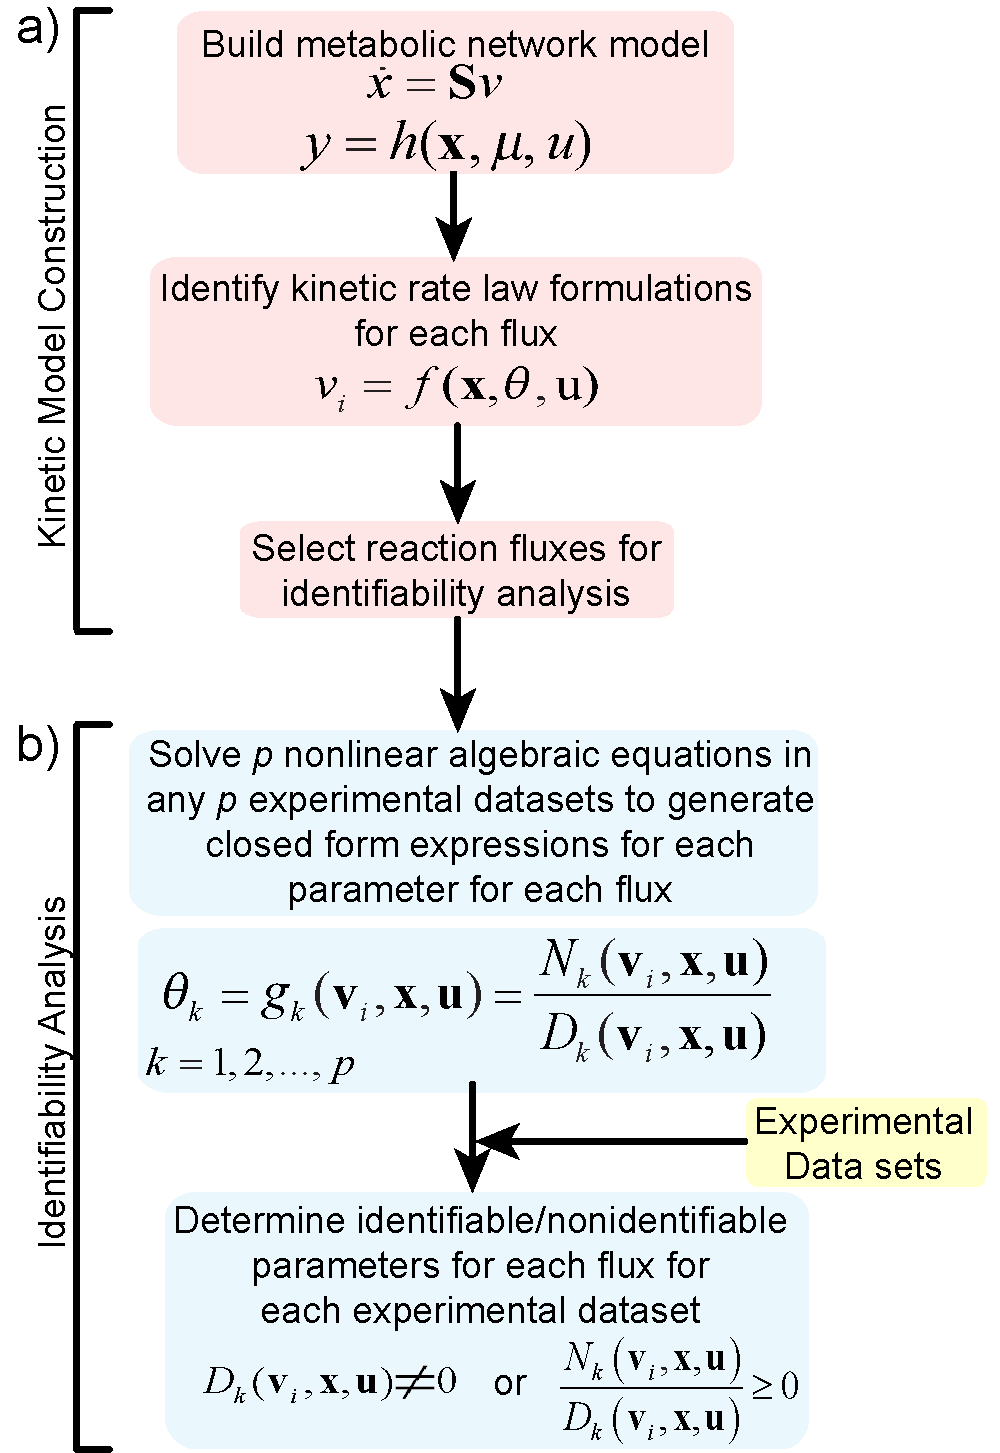
\includegraphics[width=.9\textwidth,height=.6\textheight,keepaspectratio]{figures/figure3/ident_analysis}}
		\caption{A flow diagram showing the methodology developed to establish practical identifiability of parameters in kinetic models of metabolism. a) The steps for the construction of a kinetic model of a metabolic network. The choice of rate law formulations to describe metabolic fluxes influences the identification methodology. The identifiability of parameters for each flux can be established independently. b) The steps for practical identifiability analysis for parameters of a single flux.}\label{fig:ident-flowchart}
	\end{figure}	
	
	For each flux $v_i$, $i={1, 2, ..., n_r}$, in the kinetic model, let $\mathbf{\theta} \in \mathbb{R}^p$ in Equation (\ref{eq:kinstoich}b). If data from $n_E$ experiments is available for the chosen metabolic network, as stated earlier, for each experiment $j = {1, 2, ..., n_E}$, we assume that all metabolite concentrations ($x$) and reaction fluxes ($v$) are measurable. We discuss the implications of relaxing this assumption later. The pertinent information for each experiment $j$ is available as a vector of concentrations and fluxes, $\mathbf{x}_j$ and $\mathbf{v}_j$, respectively (Figure \ref{fig:ident-flowchart}b). 
	
	In order to establish the practical identifiability of kinetic parameters for each flux $v_i$, $i={1, 2, ..., n_r}$, we describe a computer algebra-based method. The primary use of the computer algebra system is to obtain closed-form expressions for each parameter in $\mathbf{\theta}$ for each flux $v_i$ (Figure \ref{fig:ident-flowchart}b). This is done by first selecting a combination of $p\le n_E$ experimental data. The fluxes and concentrations from $p$ different experiments are then used to formulate a system of nonlinear algebraic equations in $\mathbb{R}^p$ for each flux $v_i$, shown in Equation (\ref{eq:nonlineq}). 
	\begin{align}\label{eq:nonlineq}
	v_{i, j} = f_j(\mathbf{x}_j,\mathbf{\theta}, \mathbf{u}_j) && \forall j=\{1, 2, ..., p\}\subset\{1, 2, ..., n_E\}
	\end{align}
	Here, $v_{i,j}$ refers to the value of the flux $v_i$ obtained from experiment $j$. $\mathbf{x}_j$ and $\mathbf{u}_j$ are the vector of metabolite and other input concentrations from each experiment $j$, and $\mathbf{\theta}$ is a vector in $\mathbb{R}^p$, whose elements are denoted by $\theta_k$.		
	
	Each equation in (\ref{eq:nonlineq}), indicated by the index $j$, corresponds to the kinetic rate law expression $f(x, \theta, u)$ for each $v_i$, $i={1, 2, ..., n_r}$, described in Equation (\ref{eq:kinstoich}b), written for concentrations ($\mathbf{x}_j$, $\mathbf{u}_j$) and fluxes ($v_{i,j}$) obtained from experiment $j$. Solving the system in Equation (\ref{eq:nonlineq}) results in $\mathbb{R}^p$ nonlinear expressions for each parameter $\theta_k$ in $\theta \in \mathbb{R}^p$ (Equation \ref{eq:theta-eq}), where $N(\mathbf{v}_i, \mathbf{x}, \mathbf{u})$ is the numerator of $g$, and $D(\mathbf{v}_i, \mathbf{x}, \mathbf{u})$ is the denominator of $g$ (Figure \ref{fig:ident-flowchart}b). Note that $\mathbf{v}_i$, $\mathbf{x}$ and $\mathbf{u}$ are used to denote vector of vectors of fluxes for reaction $i$ ($\mathbf{v}_i$), metabolite ($\mathbf{x}$) and input ($\mathbf{u}$) concentrations, respectively, obtained from $p$ experiments denoted by the index $j = {1, 2, ..., p}$.
	\begin{align}\label{eq:theta-eq}
	\theta_k = g_k(\mathbf{v}_i, \mathbf{x}, \mathbf{u}) = \frac{N_k(\mathbf{v}_i, \mathbf{x}, \mathbf{u})}{D_k(\mathbf{v}_i, \mathbf{x}, \mathbf{u})}
	\end{align}

	The identifiability of parameter $\theta_k$, $k = {1, 2, ..., p}$, for flux $v_i$ can be established by determining the value of $D_k(\mathbf{v}_i, \mathbf{x}, \mathbf{u})$ (Figure \ref{fig:ident-flowchart}b): any parameter $\theta_k$ is said to practically identifiable if $D_k(\mathbf{v}_i, \mathbf{x}, \mathbf{u})\neq0$, and practically non-identifiable if $D_k(\mathbf{v}_i, \mathbf{x}, \mathbf{u}) = 0$. Furthermore, the physical properties of the kinetic parameters can be used to distinguish between identifiable and non-identifiable parameter values by designating only parameters with a non-negative value of $g_k(\mathbf{v}_i, \mathbf{x}, \mathbf{u})$ as identifiable (Figure \ref{fig:ident-flowchart}b). The solution $g_k(\mathbf{v}_i, \mathbf{x}, \mathbf{u})$ in Equation (\ref{eq:theta-eq}) is unique for an identifiable $\theta_k$, and an infinite number of solutions are possible for a non-identifiable $\theta_k$. However, if there are multiple but finite solutions $g_k(\mathbf{v}_i, \mathbf{x}, \mathbf{u})$, then the corresponding parameter $\theta_k$ is locally identifiable.
	
	%For completeness, in the following sections we provide a previously published kinetic model of a small gluconeogenic network (section \ref{sec:small-model}). 
	
	\subsection{Degree of identifiability: A quantitative measure of practical identifiability}\label{sec:degree_of_identifiability}
	We express the practical identifiability of kinetic parameters using a simple quantitative term called the degree of identifiability. We describe the degree of identifiability of any single parameter as the percentage of all data combinations (used to test for practical identifiability) that can identify that parameter. 
	
	As an example, if 90\% of all the experimental data combinations used for testing can identify a parameter $\theta_i$, then the degree of identifiability of $\theta_i$ is said to be 0.9 or 90\%. On the other hand, if only 50\% of the combinations can identify another parameter $\theta_j$, then $\theta_j$ has a degree of identifiability of 0.5 or 50\%. Furthermore, we can create a hierarchy of practically identifiable parameters using their degrees of identifiability. In the above instance of the two parameters $\theta_i$ and $\theta_j$ that have degrees of identifiability of 90\% and 50\% respectively, $\theta_i$ is classified to be more identifiable than $\theta_j$ due to its relatively higher degree of identifiability. 
	
	Determining this hierarchy of identifiable parameters can help in distinguishing parameters that can be identified by any type and any combination of experiments from parameters that can be identified by only a select type and combination of experiments. Such a classification can subsequently be used to design minimal sets of experiments that can practically identify all kinetic parameters used to model a metabolic network, going from the least identifiable parameter to the most identifiable parameter.  	
	
	\subsection{Kinetic model of gluconeogenesis in \textit{E. coli}}\label{sec:small-model}
	A previously proposed kinetic model \parencite{Kotte2014, Srinivasan2017} for acetate consumption through gluconeogenesis (Figure \ref{fig:network}) is used as a case study to illustrate identifiability analysis for experimental design for parameter estimation in kinetic models of metabolism. The kinetic model is described below.
	
	\begin{figure}[!tbhp]
		\centering{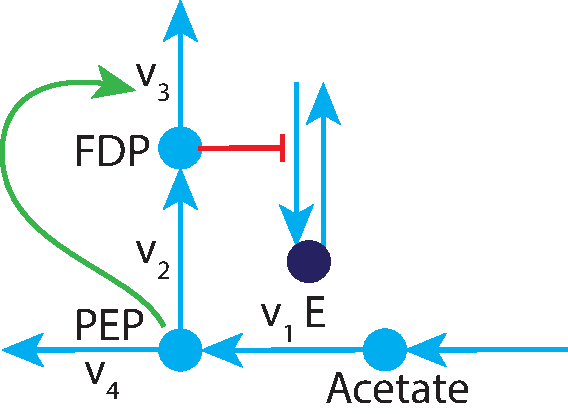
\includegraphics[width=.3\textwidth,height=.6\textheight,keepaspectratio]{figures/figure5/Figure1_NetworkA}}
		\caption{The previously published small metabolic network for gluconeogenesis used to demonstrate our practical identifiability method for kinetic models of metabolism.}\label{fig:network}
	\end{figure}		
	
	\begin{equation}\label{eq:ode1}
	\frac{d}{dt}pep=v_1-v_2-v_4
	\end{equation}
	\begin{equation}\label{eq:ode2}
	\frac{d}{dt}fdp=v_2-v_3
	\end{equation}
	\begin{equation}\label{eq:ode3}
	\frac{d}{dt}E=v_5 - d E
	\end{equation}
	The kinetic expressions for fluxes $v_1$ through $v_5$ are given below. The consumption of acetate through $v_1$ and conversion of \textit{pep} through $v_2$ are expressed in Equations (\ref{eq:flux1}) and (\ref{eq:flux2}) respectively using Michaelis-Menten kinetics. The acetate flux through $v_1$ is also governed by the quantity of available enzyme E. 
	\begin{equation}\label{eq:flux1}
	v_1 = k_{1}^{cat}E\frac{ac}{ac+K_{1}^{ac}}
	\end{equation}		
	The model for flux $v_1$ of the small network (Figure \ref{fig:network}), uses the concentration of the enzyme E as a variable (Equation \ref{eq:flux1}). Since we assume that steady state experimental information is only available for metabolite concentrations and fluxes, and not for enzymes (again the details on relaxing this assumption are discussed later), the expression in Equation (\ref{eq:flux1}) for $v_1$ cannot be used for identifying parameters $k_1^{cat}$ and $K_1^{ac}$. So, we modify the Michaelis-Menten kinetic rate law expression to eliminate the enzyme concentration E as a variable in Equation (\ref{eq:flux1a}). Consequently $k_1^{cat}$ is replaced by $V_1^{max}$ as a parameter to describe $v_1$. The corresponding enzyme binding constant is denoted as $K_1^{ac} (ne)$ to distinguish it from the enzyme binding constant calculated in the presence of measured enzyme concentration data.
	\begin{align}\label{eq:flux1a}
	v_1 = V_1^{max}\frac{ac}{ac+K_{1}^{ac}(ne)}
	\end{align}		
	We choose the expression for flux $v_1$ given in Equation (\ref{eq:flux1a}) to demonstrate our method for practical identifiability. 	
	\begin{equation}\label{eq:flux2}
	v_2 = V_{2}^{max}\frac{pep}{pep+K_{2}^{pep}}
	\end{equation}
	\begin{equation}\label{eq:flux3}
	v_3 = V_{3}^{max}\frac{\tilde{fdp}\left(1+\tilde{fdp}\right)^3}{\left(1+\tilde{fdp}\right)^4+L_3\left(1+\frac{pep}{K_{3}^{pep}}\right)^{-4}}
	\end{equation}
	The allosterically regulated flux $v_3$ for the consumption of \textit{fdp} is expressed in Equation (\ref{eq:flux3}) using the Monod-Wyman-Changeux (MWC) model for allosterically regulated enzymes, where $\tilde{fdp}$ refers to the ratio of \textit{fdp} with respect to its allosteric binding constant $K_{3}^{fdp}$. 
	
	The practically identifiability of parameters of a given flux are determined by solving a system of nonlinear algebraic equations using a computer algebra system (Section \ref{sec:ident}). We find that the nonlinearity of the MWC kinetic rate law used to model the allosteric regulation of $v_3$ makes it computationally intractable for determining the closed form expressions of the three parameters $V_3^{max}$, $K_3^{fdp}$ and $K_3^{pep}$ using a computer algebra system (Mathematica or SymPy in Python). In order to overcome this computational obstacle, we model the reaction rate for $v_3$ using the convenience kinetic rate law formulation \parencite{Liebermeister2006}. The corresponding expression obtained for $v_3$ is given below (Equation \ref{eq:flux3_convkin}). 	
	\begin{align}\label{eq:flux3_convkin}
	v_3 = V_3^{max}\left(\frac{1}{1 + \frac{K_3^{pep}}{pep}}\right)\left(\frac{\frac{fdp}{K_3^{fdp}}}{1 + \frac{fdp}{K_3^{fdp}}}\right)
	\end{align}	
	
	The flux $v_4$ for the export of \textit{pep} is expressed as a linear equation dependent on $pep$ in Equation (\ref{eq:flux4}).
	\begin{equation}\label{eq:flux4}
	v_4 = V_{4}^{max}.pep
	\end{equation}		
	The production of enzyme E is represented by flux $v_5$. The inhibition of this flux by \textit{fdp} is modeled using Hill kinetics, where $K_e^{fdp}$ represents the Hill binding constant for the inhibiting metabolite \textit{fdp}, $n_e$ is the Hill exponent, and $V_e^{max}$ is the maximum reaction rate for $v_5$.
	\begin{align}\label{eq:flux5}
	v_5 = V_e^{max}\left(\frac{1}{1+\left(\frac{fdp}{K_{e}^{fdp}}\right)^{n_e}}\right)
	\end{align}
		
	\subsection{Experimental design through practical parameter identification}\label{sec:experimental_design}		
	Not all metabolite concentrations and fluxes in the model (Equation \ref{eq:kinstoich}) change for any random experiment. This makes unambiguous estimation of parameters impossible, either due to the inherent correlation between changes in different concentrations or fluxes, or due to the homeostasis of the concentrations and fluxes under the chosen experimental conditions \parencite{Heijnen2013}. In such scenarios, the need to design experiments to effect a change in, and discriminate between changes in different concentrations/fluxes becomes necessary. 
		
	Following the methodology described in section \ref{sec:ident}, and demonstrated in section \ref{sec:example} for a single flux using data from a combination of two different experiments, all distinct combinations found based on experiments described in section \ref{sec:experiments} of the Supplementary Information can be tested for their ability to practically identify any of the three fluxes in the small metabolic network. This step would determine the degree of identifiability (defined in section \ref{sec:degree_of_identifiability}) of each parameter in each flux in the model, and help distinguish experiment combinations that contribute to identifiability from combinations that do not practically identify any parameter in the model (Figure \ref{fig:ident-flowchart}b). In doing so, it is possible to obtain a minimal and informative collection of experiments that can be performed to identify as many model parameters as possible (Figure \ref{fig:ident-design}). Consequently, the set of experiments can be used to estimate all the identifiable parameters in the model. This is formally explained below.
	
	The identifiability of each parameter based on each experiment with index $j = {1, 2, ..., n_E}$ is established based on the methodology described in section \ref{sec:ident} (Figure \ref{fig:ident-flowchart}b), and demonstrated in section \ref{sec:example}. Subsequently, for any flux $v_i$, and for any combination of $p$ experimental data sets, if the experimental concentrations and fluxes ($\mathbf{x}_j$ and $\mathbf{v}_j$, respectively, where $j = {1, 2,..., p}$) do not satisfy the condition for identifiability for any parameter $\theta_k$ in $\theta\in\mathbb{R}^p$ (Figure \ref{fig:ident-flowchart}b), then at least one of the $p$ experiments needs to be changed to make parameter $\theta_k$ identifiable. Consequently, the corresponding experiment cannot be used for estimating parameter $\theta_k$, and needs to be discarded from the set of all necessary experiments. Furthermore, another experiment from $j = {1, ..., n_E}$ needs to be selected to replace the discarded experiment such that parameter $\theta_k$ is identifiable. This process has to be repeated until all parameters in $\theta\in\mathbb{R}^p$ are identifiable for flux $v_i$. In doing so, we can arrive at a set of $p$ experiments that will always result in practically identifiable parameters for flux $v_i$. Note that if none of the $n_E$ pre-selected experiments satisfy the identifiability condition, then we can design an $(n_E+1)^{th}$ experiment that can replace one of the experiments that causes practical non-identifiability. This analysis can be performed for each flux in a metabolic network independent of all the other fluxes, making it theoretically scalable even to genome-scale models of metabolism. 	
	
	\section{Results}
	First, in Section \ref{sec:example}, we demonstrate the use of the methodology that we described in Section 2.1 to practically identify parameters in flux $v_1$ of the small gluconeogenic network (Figure \ref{fig:network}) model given in Section \ref{sec:small-model}. 
	We discuss the ability of the proposed methodology to determine the structural identifiability of parameters modeling $v_1$, $v_3$ and $v_5$ in Section \ref{sec:proof}. 	
	In Section \ref{sec:initial_analysis} that follows, we show how the demonstrated methodology is capable of practically identifying and estimating parameters for fluxes $v_1$, $v_2$, $v_3$ and $v_5$ using steady state flux values and metabolite concentrations. 
	The various ways in which this information can be used for designing experiments to generate data that can facilitate estimation of identifiable parameters are discussed in Section \ref{sec:design} that follows.
	The contribution of the uncertainty in the data (due to differences between in vivo and in vitro kinetics) towards identifying parameters in enzyme kinetic models is discussed in Section \ref{sec:uncertainty}.
		
	\subsection{Identifying parameters in kinetic models of metabolism: an example}\label{sec:example}	
	In this section, we illustrate the proposed methodology step by step to identify parameters of flux $v_1$ in the small metabolic network (Figure \ref{fig:network} and Section \ref{sec:small-model} of the Supplementary Information). We choose the expression for flux $v_1$ given in Equation (\ref{eq:flux1a}) for this demonstration. 
	\begin{align}\tag{S5}
	v_1 = V_1^{max}\frac{ac}{ac+K_{1}^{ac}(ne)}
	\end{align}		
	Since $\theta = \{V_1^{max}, K_1^{ac} (ne)\} \in \mathbb{R}^2$ for $v_1$, as mentioned in Section \ref{sec:experiments}, we need steady state concentration and flux measurements from at least two different experiments. So, from the $n_E = 21$ different experiments described in Section \ref{sec:experiments} and Table \ref{tab:pval}, we can choose multiple combinations of $p = 2$ experiments to satisfy the data requirements for identifying $v_1$ i.e., in Equation (\ref{eq:nonlineq}) $j = \{1, 2\}$. We label the available concentrations and fluxes as ${ac}^{(j)}$ and ${v_1}^{(j)}$, respectively. Then, the nonlinear algebraic equations shown in Equation (\ref{eq:nonlineq}) can be formulated for $v_1$ as:
	\begin{align*}%\label{eq:nonlin-flux2}
	{v_1}^{(j)} = V_{1}^{max}\frac{ac^{(j)}}{ac^{(j)}+K_{1}^{ac}(ne)} &&  j=\{1, 2\}
	\end{align*}
	
	Solving this simultaneous system of equations in $\mathbb{R}^2$ using Mathematica (Wolfram Research, USA), a computer algebra system, we get $p=2$ nonlinear algebraic expressions for parameters $V_1^{max}$ (Equation \ref{eq:v1_par}a) and $K_1^{ac}(ne)$ (Equation \ref{eq:v1_par}b). These expressions have the form shown in Equation (\ref{eq:theta-eq}).
	\begin{subequations}\label{eq:v1_par}
		\begin{align}		
		\theta_1 &= V_1^{max} = \frac{v_1^{(1)}v_1^{(2)}(ac^{(1)}-ac^{(2)})}{v_1^{(2)}ac^{(1)}-v_1^{(1)}ac^{(2)}}\\
		\theta_2 &= K_1^{ac}(ne) = \frac{ac^{(1)}ac^{(2)}(v_1^{(1)}-v_1^{(2)})}{v_1^{(2)}ac^{(1)}-v_1^{(1)}ac^{(2)}}
		\end{align}
	\end{subequations}
	To test the practical identifiability of the parameters in Equation \ref{eq:v1_par}, we substitute any suitable in silico experimental data and determine the value of the denominator of the right hand side expression. Since the enzyme binding constant ($K_1^{ac}(ne)$) and the maximum reaction rate ($V_1^{max}$) cannot be negative, we can further constrain the criteria for identifiability for both these parameters by saying that the evaluated expressions in Equation (\ref{eq:v1_par}) should be non-negative (Figure \ref{fig:ident-flowchart}b). The parameter values that are obtained for $V_1^{max}$ and $K_1^{ac} (ne)$ by substituting in silico steady state experimental data are shown in Supplementary Figure \ref{fig:v1_v1max_ck_values}. Due to the numerous possible parameter values seen in Supplementary Figure \ref{fig:v1_v1max_ck_values}, we can conclude that both $V_1^{max}$ and $K_1^{ac}$ are practically non-identifiable.
	
	We can also apply the proposed methodology to practically identify parameters in $v_1$ under the assumption that the protein concentration for the enzyme \textit{E} is also available, in addition to the measured metabolite concentrations and fluxes. In doing so, we get two expressions similar to the one shown in Equation (\ref{eq:v1_par}) for $k_1^{cat}$ and $K_1^{ac}$. Here, the value of $V_1^{max}$ in Equation (\ref{eq:flux1a}) is substituted with $V_1^{max} = k_1^{cat}E$ instead. The corresponding identifiability expressions for $k_1^{cat}$ and $K_1^{ac}$ are given in Equation (\ref{eq:v1_k1cat}).	
	\begin{subequations}\label{eq:v1_k1cat}
		\begin{align}
		k_1^{cat} = \frac{ v_1^{(1)}v_1^{(2)} \left( ac^{(1)}- ac^{(2)}\right)}{v_1^{(2)}ac^{(1)}E^{(1)} - v_1^{(1)}ac^{(2)}E^{(2)}}\\
		K_1^{ac} = \frac{ac^{(1)}ac^{(2)}\left(v_1^{(1)}E^{(2)} - v_1^{(2)}E^{(1)}\right)}{v_1^{(2)}ac^{(1)}E^{(1)} - v_1^{(1)}ac^{(2)}E^{(2)}}
		\end{align}
	\end{subequations}	
	We show the parameter value for $k_1^{cat}$ and $K_1^{ac}$ that are obtained through the practical identifiability analysis in Figure \ref{fig:ident_values}a when in silico experimental data is substituted in Equation (\ref{eq:v1_k1cat}). Through Equation (\ref{eq:v1_k1cat}) and Figure \ref{fig:ident_values}a we are able to show that the uncertainty in the parameter estimates (Supplementary Figure \ref{fig:v1_v1max_ck_values}) can be resolved through the incorporation of the available enzyme concentrations. Thus, having more experimental information can help resolve practical identifiability.
	
	\begin{figure}[!tbhp]
		\centering{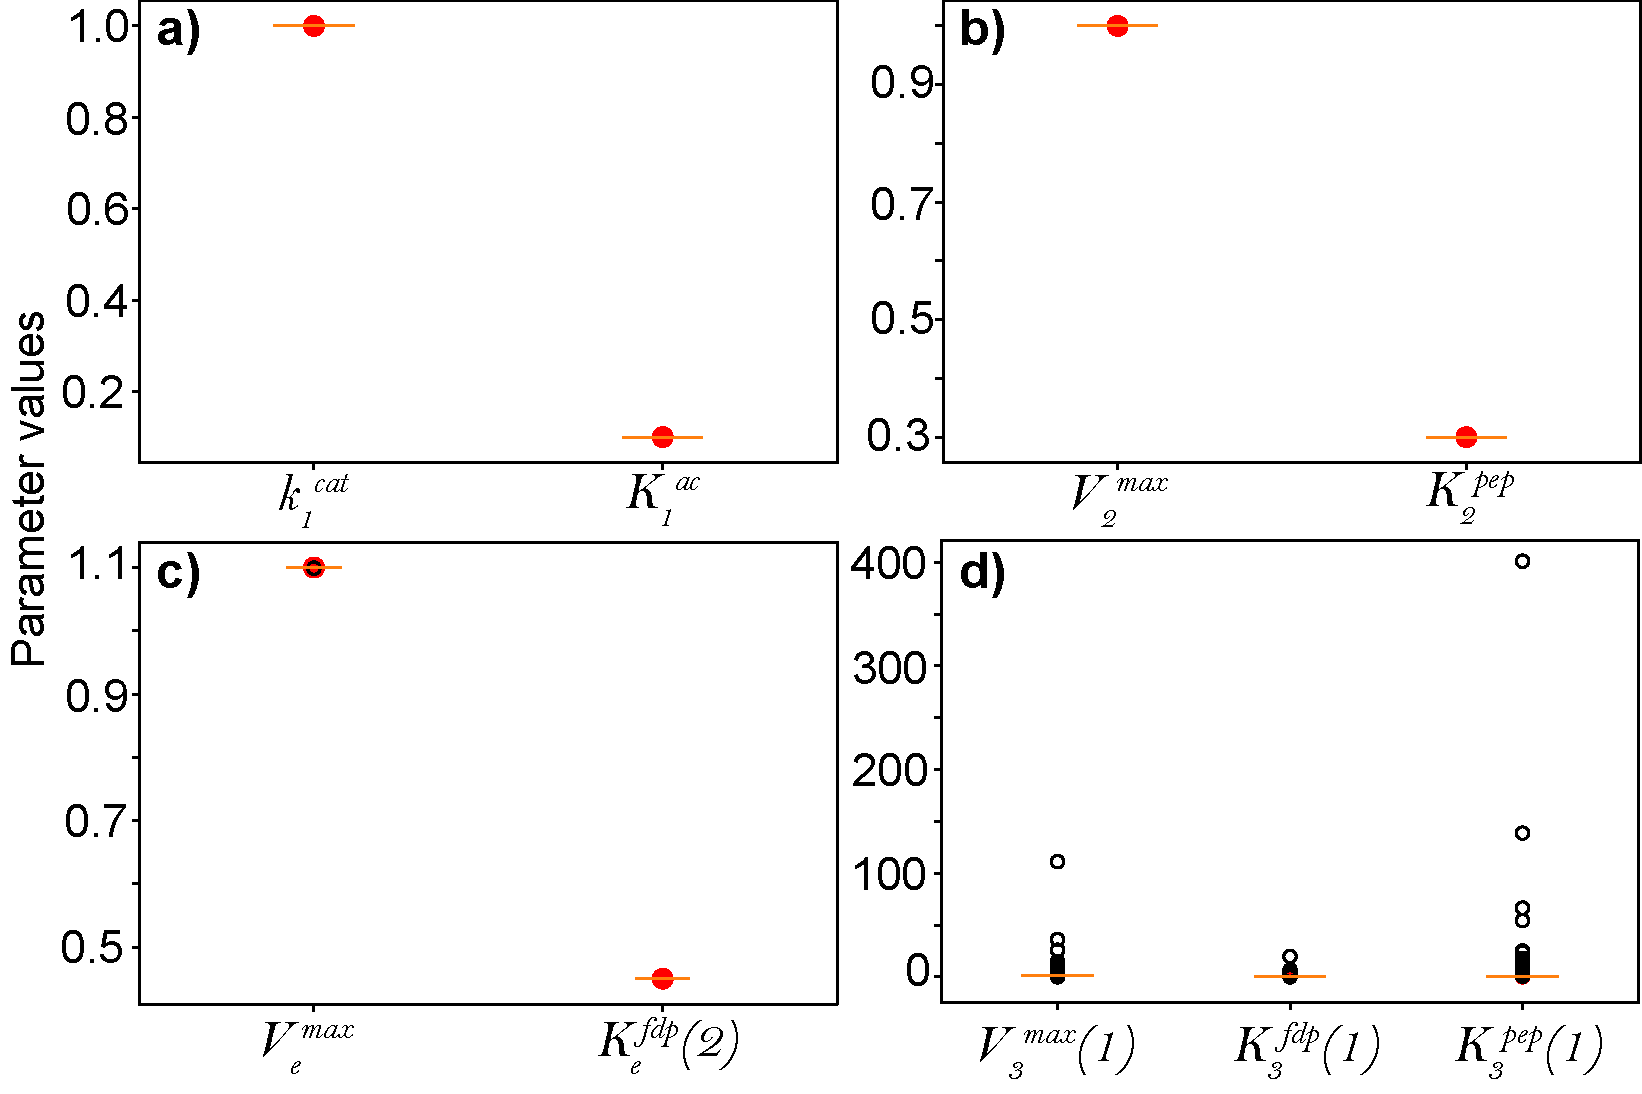
\includegraphics[width=.8\textwidth,height=.6\textheight,keepaspectratio]{figures/figure6/v1_k1cat_v2_v5_2_v3_ck_1_parameter_values}}
		\caption{Distribution of predicted parameter values when performing practical identifiability analysis using closed-form solutions for each parameter in flux a) $v_1$, b) $v_2$, c) $v_5$, and d)$v_3$. For $v_1$, we have assumed that enzyme concentration is available and have accordingly identified and estimated $k_1^{cat}$, as opposed to $V_1^{max}$. The parameter values for only the second root of $K_e^{fdp}$ in $v_5$ ($K_e^{fdp}(2)$) is shown, since $K_e^{fdp}(1)$ is not estimated by any combination of two experiments, and $V_e^{max}$ is estimated by all combinations. Only one of the two roots for $v_3$ is shown in panel d. The estimated data for the second root has a similar distribution to that of the first root and is shown in the Supplementary Information. Data is generated using the Convenience Kinetic model for allosteric regulation for $v_3$.}\label{fig:ident_values}
	\end{figure}
	
	In the following section we present results from the identifiability analysis of fluxes $v_2$, $v_3$ and $v_5$ in the small metabolic network (Figure \ref{fig:network}), using the methodology (Figure \ref{fig:ident-flowchart}) that we have demonstrated above for $v_1$. 
	
	\subsection{Establishing Structural identifiability of parameters based on closed-form solutions}\label{sec:proof}
	As mentioned in Section \ref{sec:ident_def}, by definition, unique parameter values based on the model structure are possible for any structurally identifiable parameter. Also, for the proposed methodology (Figure \ref{fig:ident-flowchart}) to work, it should be possible to obtain closed form solutions for each parameter in the enzyme kinetic model for each flux as shown in Equation (\ref{eq:theta-eq}). Since the ability to obtain closed-form solutions for each parameter is dependent on the model structure, any parameter that has non-unique closed-form solutions can be called a structurally non-identifiable parameter. However, if the number of solutions that the parameter has are finite, then the parameter is only locally structurally identifiable. 
	
	We demonstrated the structural identifiability of parameters modeling $v_1$ in Section \ref{sec:example}. We have shown that the parameters have only one unique closed-form solution, and accordingly are structurally identifiable. Since $v_2$ is also expressed using the Michaelis-Menten model, just like $v_1$, we find that the parameters ($V_2^{max}$ and $K_2^{pep}$) are also structurally identifiable. The closed-form expressions for these parameters are similar to the ones shown in Equation \ref{eq:v1_par}, with \textit{ac} replaced by \textit{pep}, and $v_1$ replaced by $v_2$. 
	
	However, we find that the parameters used to model $v_3$ using the Convenience kinetics rate law, and $v_5$ using the Hill kinetic rate law are not structural identifiable under certain conditions. First, for $v_3$, we find that the parameters $V_3^{max}$, $K_3^{fdp}$ and $K_3^{pep}$ have two different closed-form solutions. Thus, based on the presence of non-unique but finite number of possible solutions for these parameters we can classify $v_3$ as a locally structurally identifiable flux. 
	
	We would like to point out that we used the Convenience kinetics rate law model for $v_3$ due to the inability of the computer algebra system to generate closed-form expressions for parameters in the Monod-Wyman-Chageaux model (Section \ref{sec:small-model}). However, we find that the Convenience kinetics model is not structurally identifiable in its current form. In order to alleviate this issue, we reduced the dimension of the parameter space for $v_3$. Originally, $\theta \in \mathbb{R}^3$ for $v_3$. By reducing the dimension of $\theta$ to $\mathbb{R}^2$, we were able to obtain a structurally identifiable model for $v_3$. To reduce the dimension of the parameter space for $v_3$, we fix either $K_3^{fdp}$ or $K_3^{pep}$ as a known quantity, and identify the other unfixed parameter along with $V_3^{max}$. This results in unique closed-form expressions for both $V_3^{max}$ and the other unfixed parameter ($K_3^{pep}$ or $K_3^{fdp}$).
	
	While $v_3$ is an allosterically regulated metabolic flux, $v_5$ describes a transcription/translation reaction using Hill kinetics. We apply our proposed methodology to identify parameters modeling $v_5$ using only the available experimental data on the metabolite concentrations and the fluxes within the metabolic network. We could not obtain closed form solutions for parameters $V_e^{max}$, $K_e^{fdp}$ and $n_e$ in $v_5$ using the computer algebra system. So, instead of changing the model as we did for $v_3$, we resorted to reducing the dimension of the parameter space by fixing one of the three parameters, the Hill coefficient $n_e$. We illustrated this for reducing the parameter space of the Convenience kinetic model for $v_3$ earlier. With a fixed and known $n_e$, $K_e^{fdp}$ has two possible closed-form solutions, making it a locally structurally identifiable parameter. On the other hand, $V_e^{max}$ has only one unique closed-form solution, and therefore is structurally identifiable. 
	
	With this we have established conditions for structural identifiability of all the major fluxes in the small metabolic network (Figure \ref{fig:network}). We have shown how our proposed methodology can be used to establish conditions for structural identifiability using steady state information on the model variables. We next discuss the practical identifiability of the parameters in $v_2$, $v_3$ and $v_5$ whose parameters are structurally identifiable only under certain conditions. 
	
	\subsection{Relationship between structural and practical parameter identifiability}\label{sec:initial_analysis}
	Together with the definition for structural identifiability we presented in Section \ref{sec:ident_def}, we also introduced the concept of practical parameter identifiability. To recall, we mentioned that  it should be possible to estimate unique parameter values based on all available experimental data for any practically identifiable parameter. As shown in Figure \ref{fig:ident-flowchart} and illustrated for $v_1$ in Section \ref{sec:example}, to determine the practical identifiability of parameters we test for the existence of a non-zero denominator of the closed-form expressions of the parameters. We also reduce the possible space within which a parameter could be practically identifiable by checking for the physiological feasibility of the parameter values that are obtained through this analysis (Figure \ref{fig:ident-flowchart}b). If the resulting parameter values obtained from various combinations of experimental data for each closed-form expression are unique, then the parameter is practically identifiable. However, if a non-unique number of parameter values are possible from multiple combinations of experimental steady state data, then the parameter is said to be practically non-identifiable. In conjunction with the conditions for structural identifiability demonstrated earlier in Section \ref{sec:proof}, if the parameter has only one unique closed-form expression, and its value is also unique, then the parameter is both structurally and practically identifiable. If either of these conditions are not satisfied, the parameters can be either locally structurally or practically identifiable or non-identifiable.
	
	Accordingly, both $v_1$ and $v_2$ are not only structurally identifiable due to the presence of unique closed-form expressions for their parameters, they are also practically identifiable because the parameters in the respective models possess unique values based on distinct combinations of experimental data (Figure \ref{fig:ident_values}a and b). 
	
	Regarding $v_5$, we showed earlier in Section \ref{sec:proof} that the identifiability of $v_5$ can be analyzed only when the Hill coefficient $n_e$ is held constant. So, in subsequent discussions, the dimension of the $v_5$ parameter space is kept at $\mathbb{R}^2$ by fixing the value of $n_e$. Under these conditions, we find that the structurally identifiable parameter $V_e^{max}$ is also practically identifiable, i.e., it has only one unique value based on all available in silico experimental data (Figure \ref{fig:ident_values}c). However, recall that unlike $V_e^{max}$, $K_e^{fdp}$ is only locally structurally identifiable as $K_e^{fdp}$ has two possible closed-form expressions. Nonetheless, despite its local structural identifiability, we find that the $K_e^{fdp}$ is also practically identifiable, like $V_e^{max}$, with only one unique parameter value (Figure \ref{fig:ident_values}c).
	
	We find that the practical identifiability of $v_5$, despite the local structural identifiability of one of its parameters, is due to the enforcement of the physiological relevance criteria on the parameters i.e., only one of the two closed-form expressions for $K_e^{fdp}$ is physiologically relevant. The other solution always acquires a negative value that has to physiological meaning. Thus, by reducing the practically identifiable space of parameters, we have shown that our methodology can establish global practical identifiability even when the parameters are only locally structurally identifiable. 
	
	Similar to $K_e^{fdp}$ in $v_5$, we also explained the local structural identifiability of $V_3^{max}$, $K_3^{fdp}$ and $K_3^{pep}$ modeling $v_3$ in Section \ref{sec:proof}. These parameters have two possible closed-form expressions. In Figure \ref{fig:ident_values}d we show that the numerical values for one of the two possible solutions for $V_3^{max}$, $K_3^{fdp}$ and $K_3^{pep}$. The numerical values for the other root of the three parameters is presented in Supplementary Figure, and they have a similar distribution. Based on the prior definition we discussed for practically identifiable parameters, the numerous possible values that the three parameters can acquire (Figure \ref{fig:ident_values}d) lead us to conclude that the parameters in $v_3$ are practically non-identifiable when they are only structurally locally identifiable. Note that these parameters are practically non-identifiable even after the reduction in the practically identifiable parameter space through application of the physiological relevance constraint (Figure \ref{fig:ident-flowchart}b). 	
	
	\begin{figure}[!tbhp]
		\centering{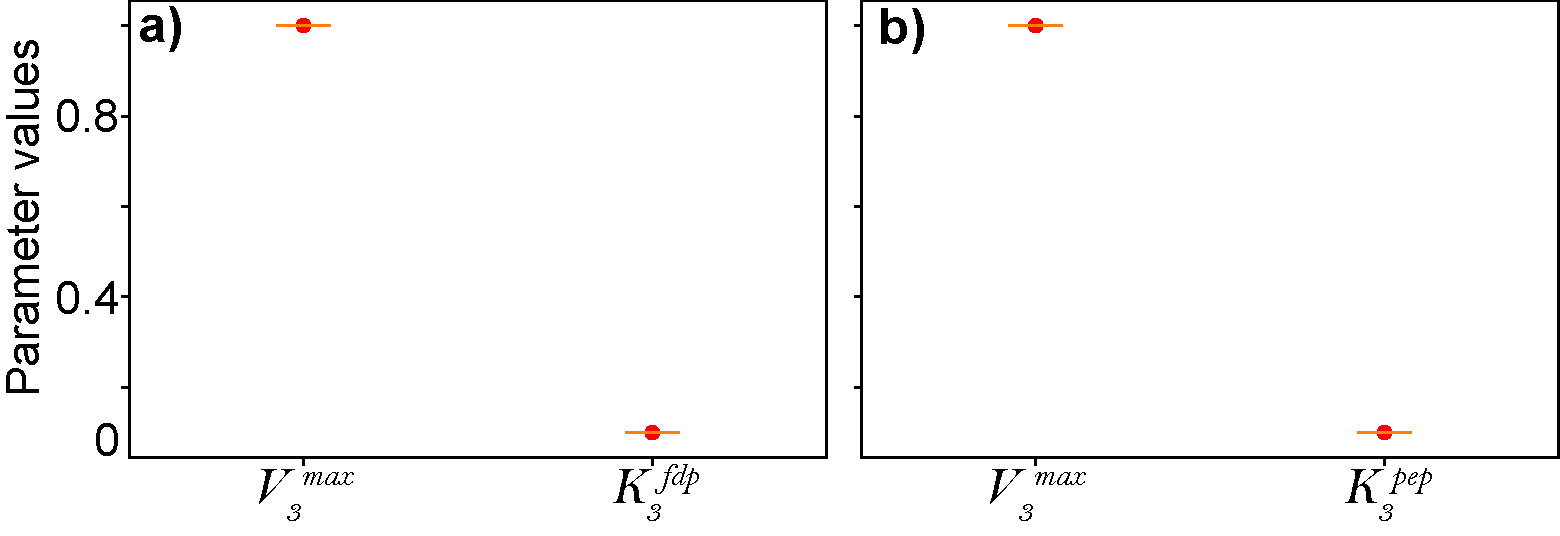
\includegraphics[width=0.8\textwidth,height=0.3\textheight, keepaspectratio]{figures/figure6/v3_var_1_2_ck_parameter_value}}
		\caption{Distribution of predicted parameter values when performing practical identifiability analysis using closed-form solutions for each parameter in flux $v_3$. The globally identifiable parameter values of a)  $V_3^{max}$ and $K_3^{fdp}$ when $K_3^{pep}$ is held constant, and b) $V_3^{max}$ and $K_3^{pep}$ when $K_3^{fdp}$ is held constant.}\label{fig:v3_var_ck_values}
	\end{figure}	

	So, the observation of practical non-identifiability for $v_3$ in the presence of local structural identifiability is in contrast to what we observed for $v_5$ earlier. However, we find that $v_3$ is practically identifiable when its parameters are also structurally identifiable (Figure \ref{fig:v3_var_ck_values}). Earlier in Section \ref{sec:proof} we had mentioned that $V_3^{max}$ and $K_3^{fdp}$ are structurally identifiable only when $K_3^{pep}$ is fixed, and $V_3^{max}$ and $K_3^{pep}$ are structurally identifiable when $K_3^{fdp}$ is fixed. Under these scenarios we find the structurally identifiable parameters to also be practically identifiable (Figure \ref{fig:v3_var_ck_values}).	
	
	Thus, in conjunction with the practical identifiability of $v_5$ established earlier, we see that it is possible to delineate between structural and practical identifiability of parameters in kinetic models of metabolism only under certain conditions, and not in others.
	
	\subsection{A priori experimental design through practical parameter identification}\label{sec:design}	
	Final section talking about distribution of experiments to obtain informative data.
	
	If the denominator of the closed-form expression is zero, then the experimental data set concerned is said to be incapable of practically identifying the said parameter, and the data from that combination of experiments is considered non-informative.
	
	In addition, we also reduce the possible space within which a parameter could be practically identifiable by checking for the physiological feasibility of the parameter values that are obtained through this analysis (Figure \ref{fig:ident-flowchart}b). If the resulting parameter values obtained from various combinations of experimental data for each closed-form expression are not physiologically feasible, then the experimental data set concerned is said to be incapable of practically identifying the said parameter, and the data from that combination of experiments is considered non-informative.
	
	
	\subsection{Parameter non-identifiability due to uncertainty in Experimental Data}\label{sec:uncertainty}
	
	
	This will cover issues related to the model used for v3. Convenience kientic model vs MWC model for data generation. Should this uncertainty also include noise?			
	
	
	
	\section{Discussions}\label{sec:discussion}	
	Parameter estimation for kinetic models has always focused on the ability to estimate parameters from existing data without the need for additional experiments, which might not be always possible if parameters are not identifiable from existing experimental data. The presence of noise is typically said to be a significant factor that results in non-identifiability. However, there different reasons for non-identifiability of parameters that we show with our work. First, non-identifiability could be structural to the model used to represent the flux, and cannot be alleviated without reduction in the parameter space. Otherwise, non-identifiability of parameters can be attributed to the lack of information about the dynamics of the system whose parameters are being estimated within the chosen experimental data. The informativeness of experiments can be tied back to their ability to discriminate the dynamics of the system under two or more different input conditions. Thus, the presence of noise only serves to exacerbate the inability of experiments to discriminate the dynamics of the systems. 
	
	Previously, methods have been developed for practical parameter identification and experimental design for kinetic models of metabolism. These methods for experimental design based on practical identification of parameters rely on solving nonlinear least squares problems using optimization approaches that cannot guarantee global optimal solutions \parencite{Raue2009a}, or calculating the Fischer Information Matrix (FIM) to obtain information on the structural and practical identifiability of parameters in kinetic models. Either of these types of methods become computationally cumbersome for models of large genome-scale, or even central carbon scale metabolic networks. Some authors have eschewed deterministic parameter estimation techniques in favour of Bayesian methods based on probabilistic estimation of parameters and experimental design \parencite{Saa2016, Saa2016a} that has the possibility of overcoming some of the issues with the deterministic techniques. 	
	 
	In this document, we have presented a scalable method to practically identify parameters in kinetic models of metabolism, and use it to design experiments that are minimal and informative for estimating the parameters that does not require solutions to non-convex optimization problems. By establishing identifiability for each flux within a metabolic network individually, we hope to overcome the scalability obstacle. Furthermore, we believe our method offers an algorithmic alternative to determine persistently excitable experiments that can enable identification of all fluxes within a metabolic network. Using a small metabolic network for gluconeogenesis, we have demonstrated that the identifiability of parameters for a given flux is dependent on the position of the flux within the metabolic network. We have also shown the ability to use our analysis to design the minimal number of experiments that are most informative for identifying all fluxes within a metabolic network.
	
	We find that the identifiability of parameters in kinetic models of metabolism using steady state information is dependent on the kinetic rate law used to model the fluxes within metabolism. The impact of the formulation and nonlinearity of a kinetic rate law expression affecting the practical identifiability of parameters in the expression may not be an unique problem isolated to the system that we are investigating. Complicated expressions for describing fluxes have been extensively used to model observed experimental data for different fluxes in a variety of organisms \parencite{Chassagnole2002a, Peskov2012, VanHeerden2014}. However, authors have favored working with approximate kinetic models of metabolism whose parameters are easily identifiable and estimable instead of trying to establish the identifiability of the parameters used in these models \textcolor{red}{(mention Heijnen papers on resolving identifiability using approximate models here)}.	
	
	We have shown that in some instances (e.g., $v_5$) local practical identifiability could be resolved to obtain global practical identifiability using constraints on the values of the parameters such that they are physically relevant. We have also shown that the structural identifiability of the parameters in any given kinetic rate law model has a bearing on the ability to determine the practical identifiability of parameters using steady state metabolomic, fluxomic and proteomic information. We find that these can sometimes be resolved by reducing the dimension of the parameter space that is being identified: $\theta \in \mathbb{R}^3$ to $\theta \in \mathbb{R}^2$ for both $v_3$ and $v_2$. Additionally, we would also like to point out that discrepancies between in vivo kinetic rate law from which typical experimental data is obtained, and the in vitro rate law used in kinetic models can itself lead to practical parameter non-identifiability or local identifiability. This can lead to uncertainty in parameter estimates made from in vivo experimental data.
	
	Our work adds to this existing body of work wherein we develop a method for practical identifiability tailored for use with nonlinear enzyme kinetic rate laws that are typically used to model fluxes in metabolic networks. With our work we hope to change the status quo in the application of systems identification techniques for kinetic models of metabolic networks. Our methodology fills the niche gap of experimental design for parameter estimation by providing a way to design informative experiments to obtain data required for parameter estimation by spending the least amount of resources.	
	In the future, we believe our work can be extended and formulated as a mixed integer linear programming problem that can be solved to determine the type and total minimum number of experiments necessary to estimate all parameters in kinetic models of genome-scale metabolic networks.
	
	%Nonetheless, all these explanations could only be verified due to the fact that the conditions for identifiability for both $v_1$ and $v_2$ are simple and readable due to the use of the Michaelis-Menten rate law to model these fluxes. Instead, in addition to presence of an allosteric interaction, when the convenience kinetic rate law is used to model this activation in $v_3$, we find that the complex expressions obtained for the three parameters preclude such an in-depth insight into the nature of persistently excitable experiments to identify  $v_3$. Thus, the only avenue through which experiments can be designed for the identification of parameters of $v_3$ would be through our proposed methodology wherein manual curation of experimental combinations required for identifiability are not necessary. 		
	
	%Based on the results we obtained in establishing the identifiability of parameters modeling all the fluxes of a small metabolic network, in the future we hope to extend this methodology to a larger metabolic network with more reactions.
	%Apart from determining experiments that are informative enough to identify parameters for each flux in a kinetic model, experimental design can also be used to design and develop a minimal set of experiments that informative enough to estimate all parameters in a metabolic network model. However, there is not only a scarcity of experimental design methods in literature devoted to the purpose of designing experiments for parameter identifiability in kinetic models of metabolism, the motivation to develop such methods is not well understood. 	
	
	\printbibliography
	
	\clearpage
	\section{Tables, Figures and Figure Captions:}
	
	
	\begin{figure}[!tbhp]
		\centering{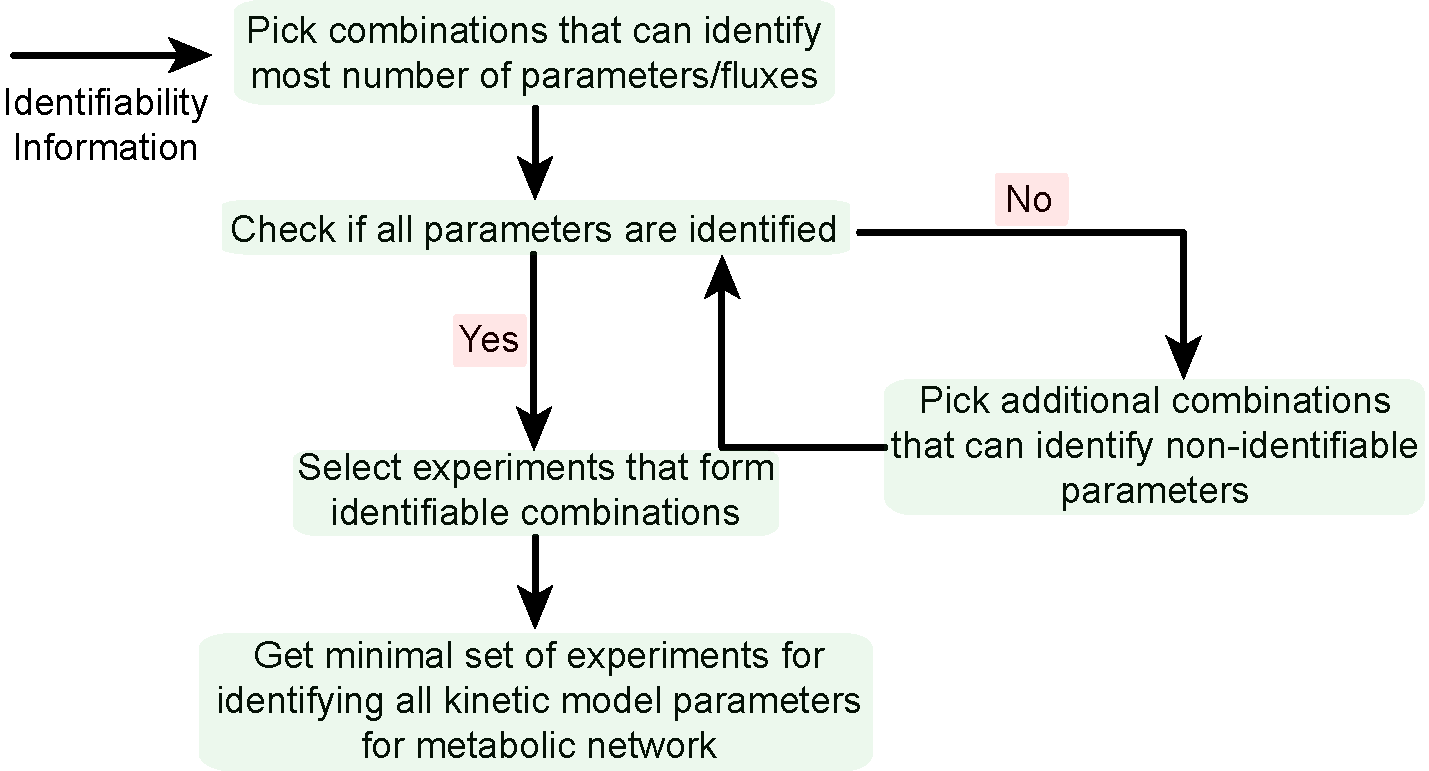
\includegraphics[width=1.0\textwidth,height=1.0\textheight,keepaspectratio]{figures/figure3/experimental_design}}
		\caption{Flow diagram showing a method for experimental design that uses our methodology for practical identification of parameters to determine the number and type of experiments required to identify all fluxes within a given metabolic network.}\label{fig:ident-design}
	\end{figure}

	\begin{figure}[!tbhp]
		\centering{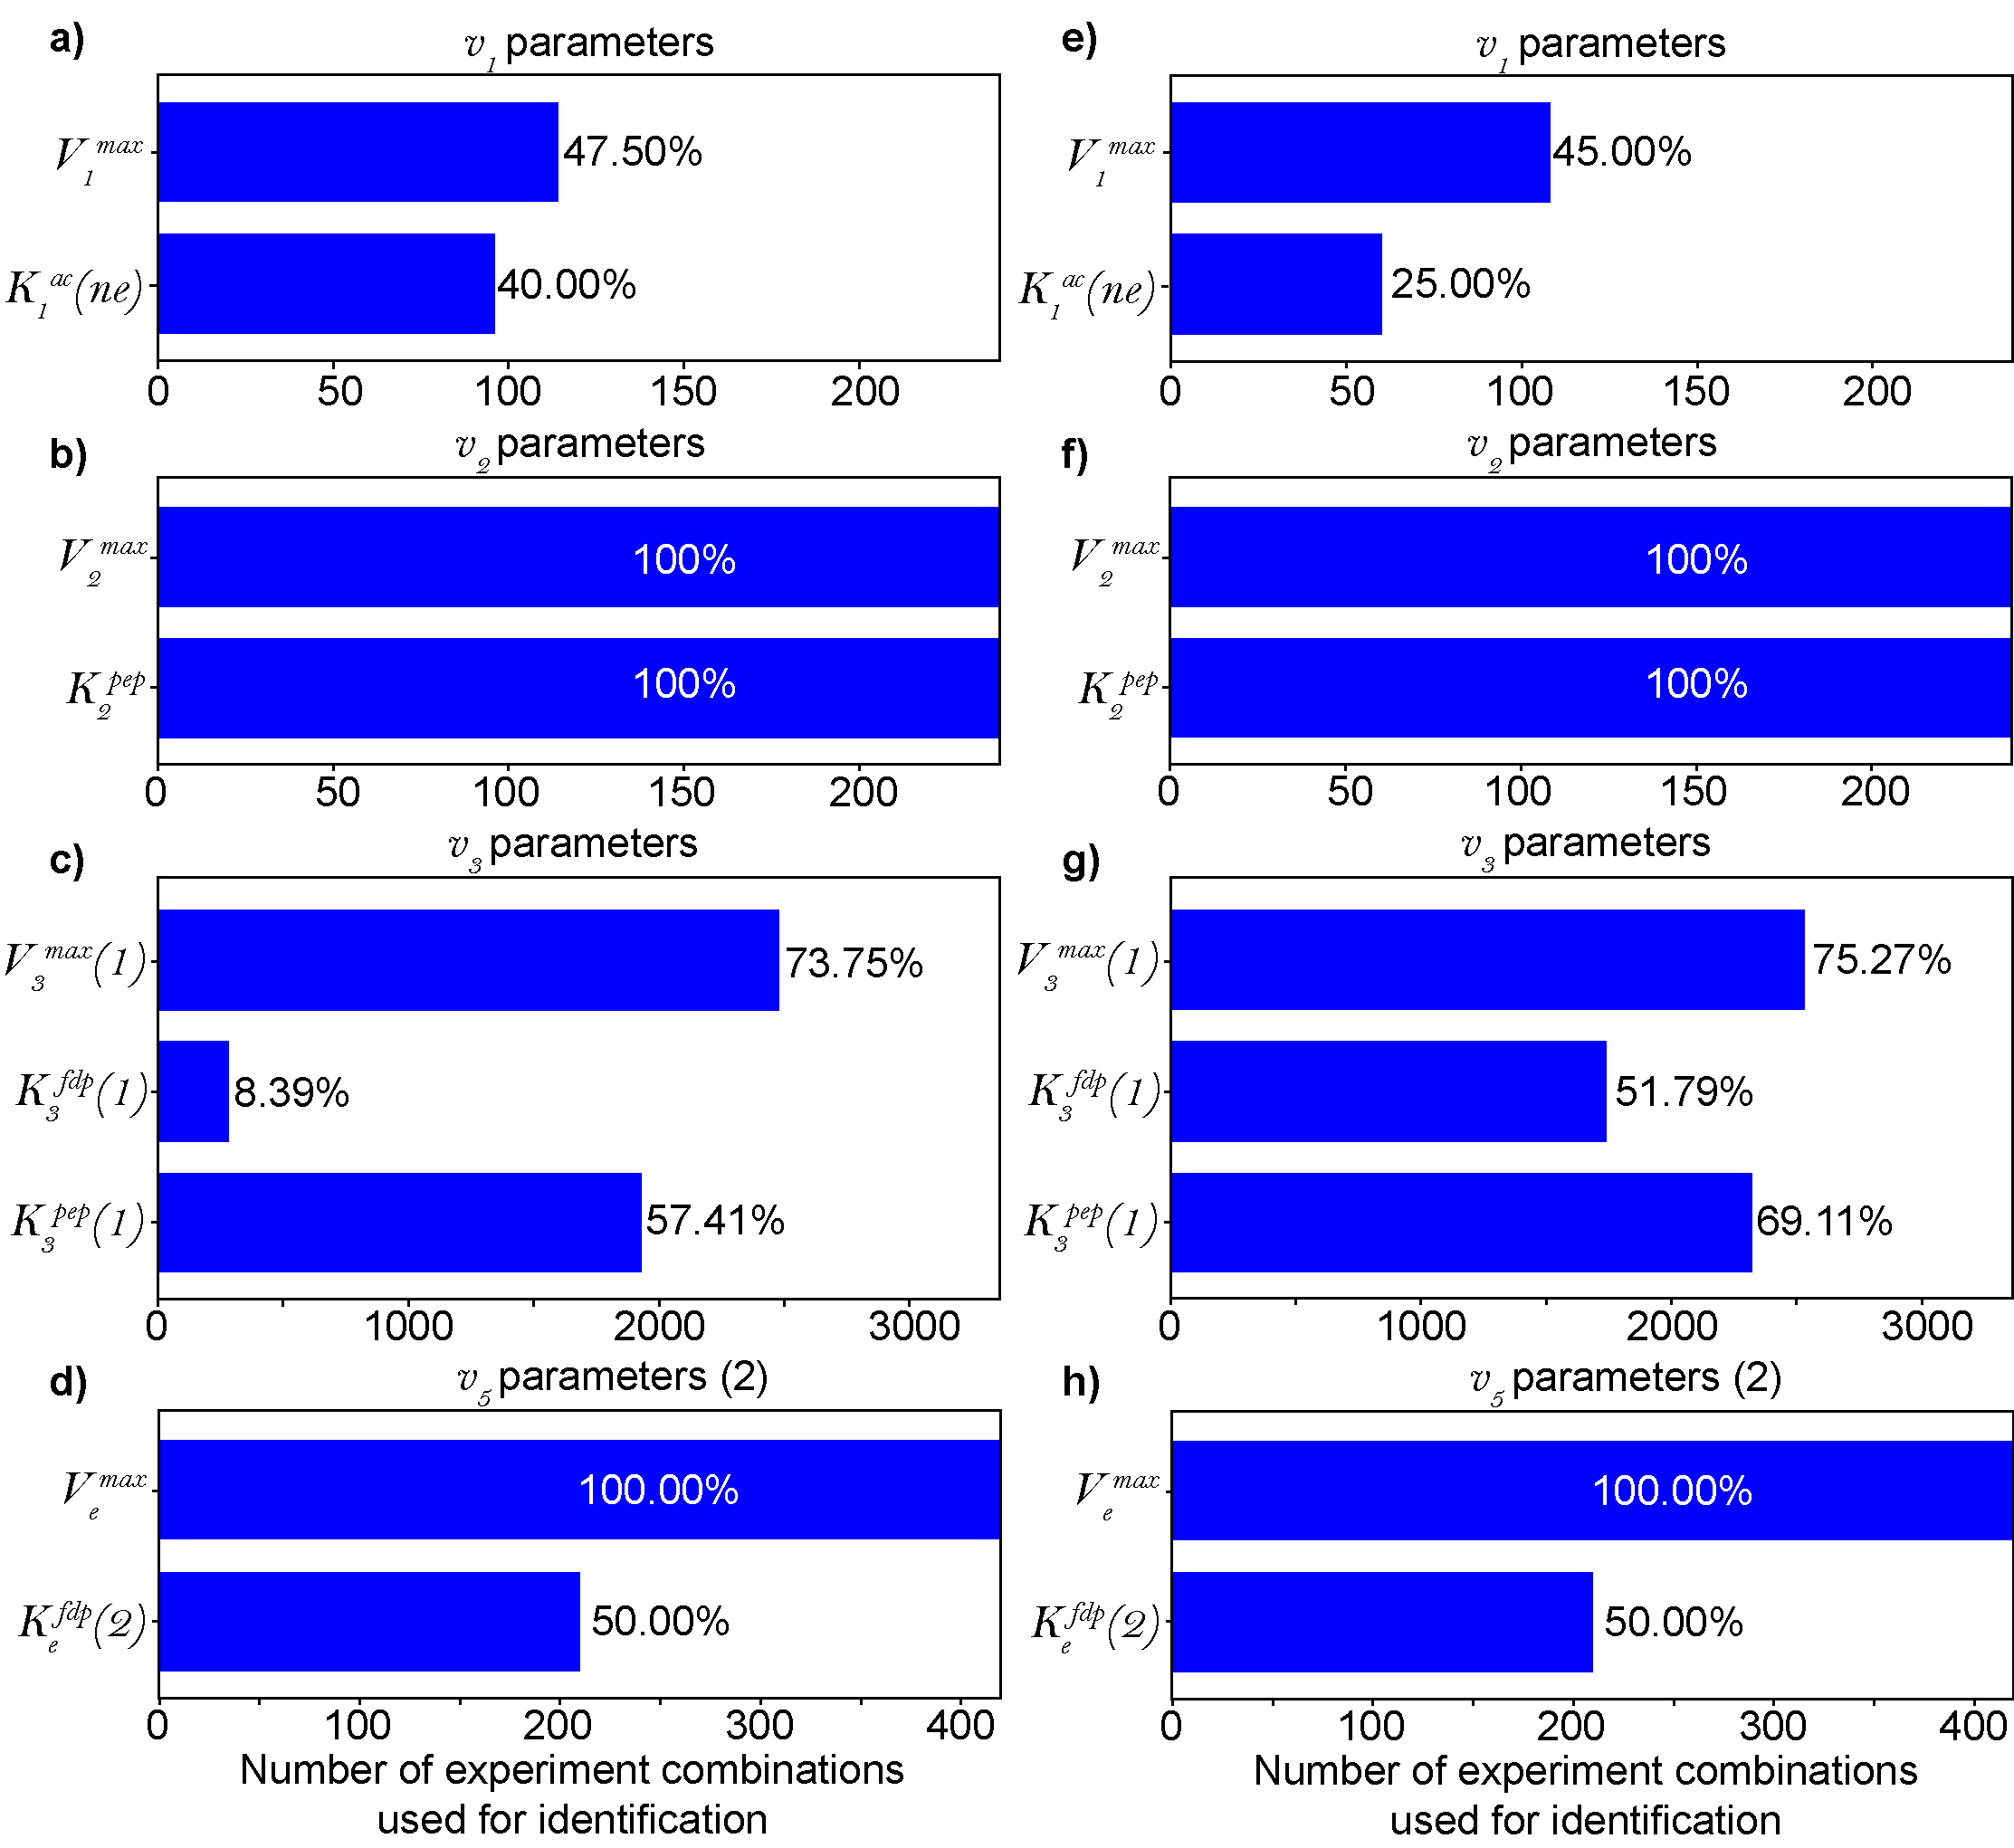
\includegraphics[width=1.0\textwidth,height=0.7\textheight,keepaspectratio]{figures/figure1/v1_V1max_v2_v3_1_v5_mwc_ck_ident}}
		\caption{The number of data combination from 21 different in silico experiments that can practically identify each parameter in fluxes a) and e) $v_1$, b)  and f) $v_2$, c) and g) $v_3$, and d) and h) $v_5$ when there is no noise in the input experimental data. The percentage of total combinations of experimental data used for analysis (240 for $v_1$ and $v_2$, 3360 for $v_3$ and 421 for $v_5$) that can identify each parameter is also specified. $v_1$, $v_2$ and $v_5$ require data from two experiments for analysis, and $v_3$ requires data from three experiments. Results for only one of the two possible roots are shown for $v_3$ and $K_e^{fdp}$ in $v_5$. The results obtained using data from the MWC model for $v_3$ are presented in the panels on the left hand side column and the panels on the right hand column show results obtained using data derived from the Convenience kinetics model for $v_3$.}\label{fig:ident}
	\end{figure}

	\begin{figure}[!tbhp]
		\centering{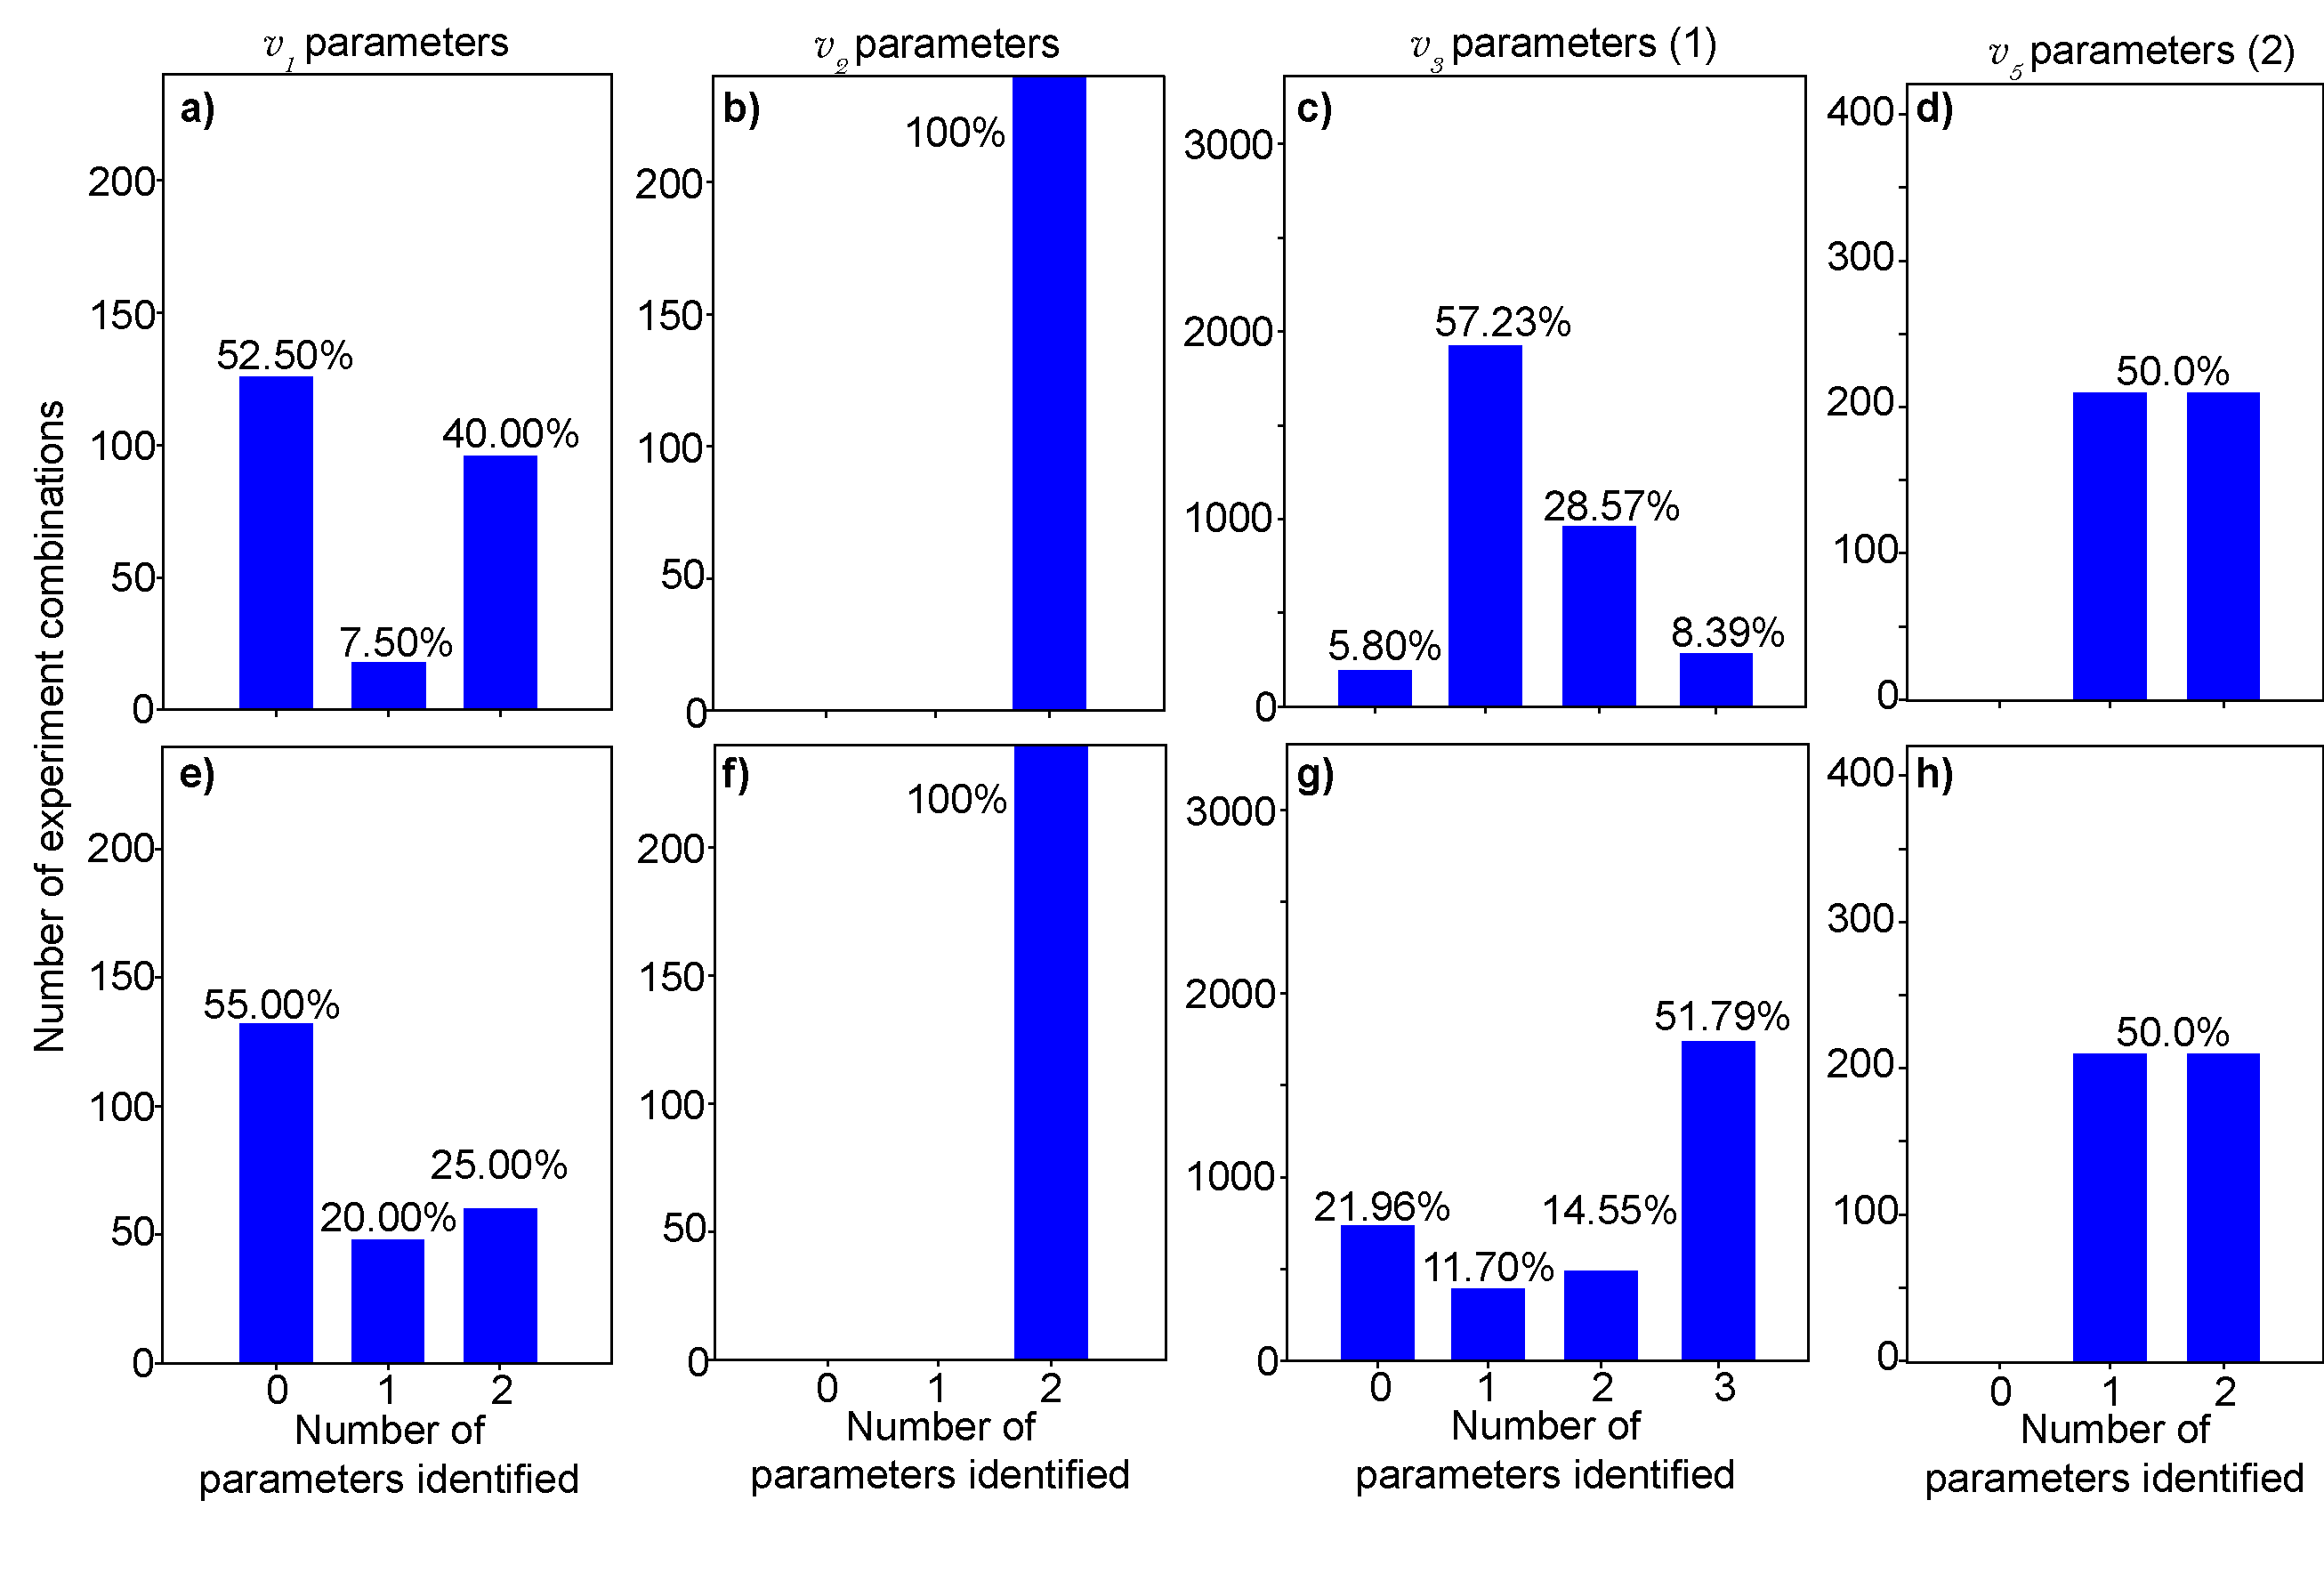
\includegraphics[width=1.0\textwidth,height=0.5\textheight,keepaspectratio]{figures/figure4/v1_V1max_v2_v3_1_v5_2_mwc_ck_data_utility}}
		\caption{Utility of experimental data combinations on the basis of their ability to identify the most number of parameters. Information is shown for parameters modeling fluxes a) $v_1$, b) $v_2$, c) $v_3$ and d) $v_5$. The total number of combinations of experimental data is shown in the vertical axis and the horizontal axis shows the total possible number of parameters that can be identified by data from combinations of a) two, b) two, c) three and d) two experiments. The percentages shown in the plots represent the fraction of the total combinations used to test identifiability of parameters for a given flux. A total of 240 data combinations are used for identifiability analysis for a) $v_1$ and b) $v_2$, 3360 combinations are used to practically identify c) $v_3$, and 420 combinations are used to analyze the identifiability of d) $v_5$. Section \ref{sec:experiments} provides more details on how the combinations of experimental data are generated.}\label{fig:data_utility}
	\end{figure}	

	\begin{figure}[!tbhp]
		\centering{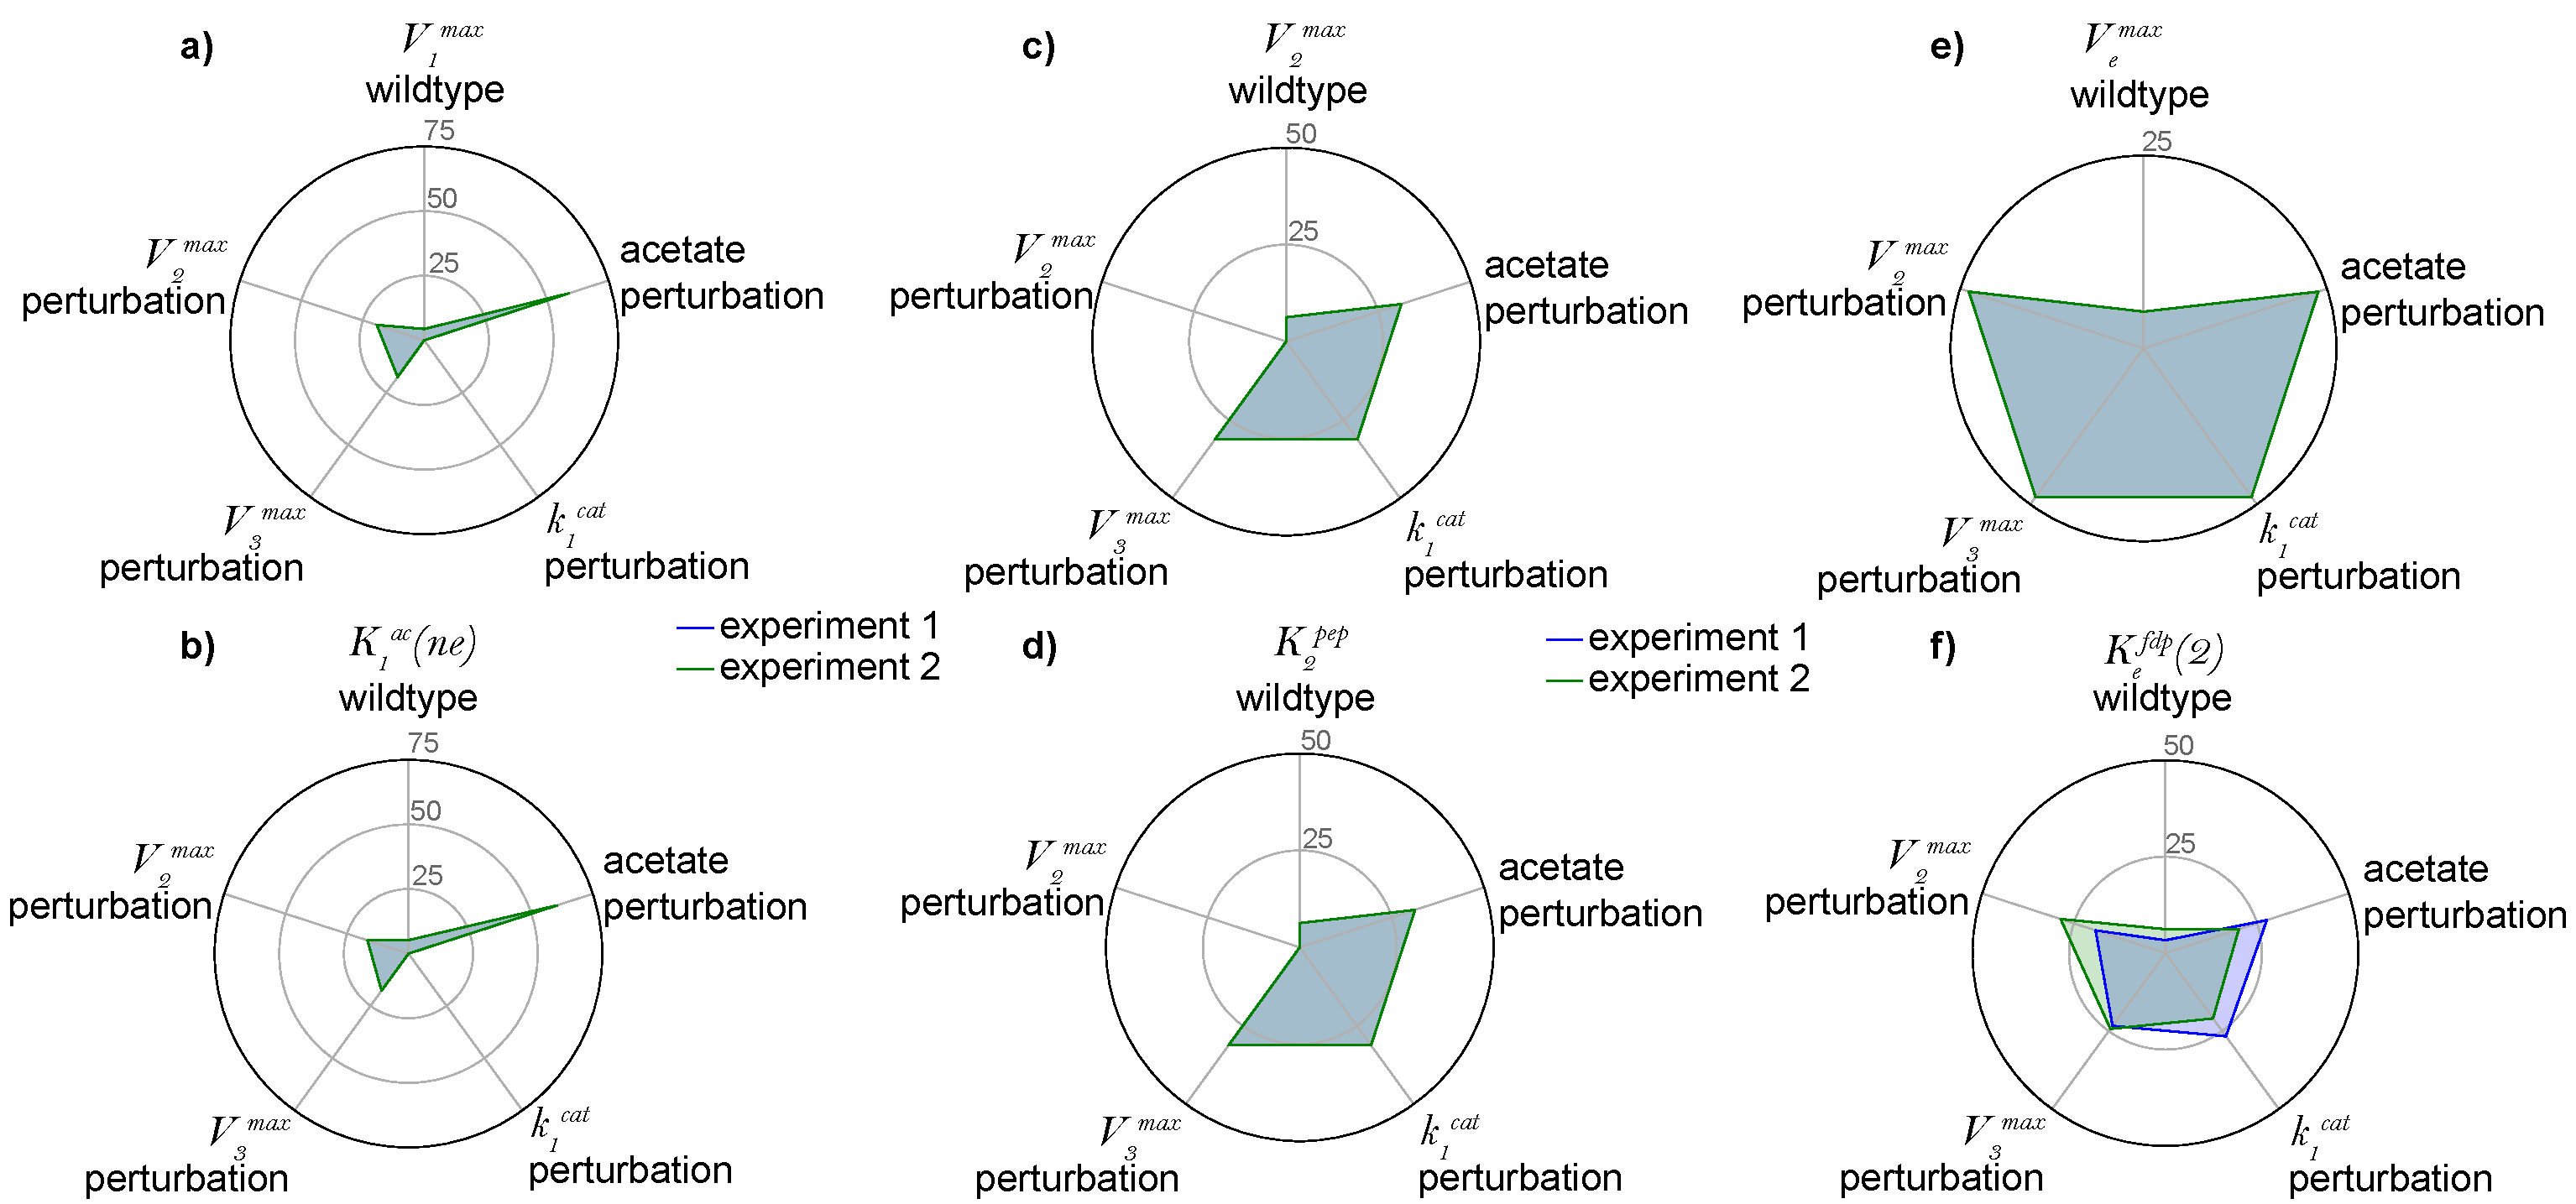
\includegraphics[width=1.0\textwidth,height=0.6\textheight, keepaspectratio]{figures/figure2/v1_V1max_v2_v5_2_exp_info}}
		\caption{The contribution of different experiments types used in a combination of two experiments ($j = \{1, 2\}$) that can practically identify parameter a) $V_1^{max}$, b) $K_1^{ac}$, c) $V_2^{max}$, d) $K_2^{pep}$, e) $V_e^{max}$ and f) $K_e^{fdp}(2)$. The percentages reflect the fractional contribution of each experiment type towards all identifiable data combinations.}\label{fig:exp_info}
	\end{figure} 
	
	\clearpage	

	\section{Old Figures, Figure Captions and other miscellaneous text}	
	Methods and tools for structural identification of parameters based on differential algebra \parencite{Ljung1994, Audoly2001, Bellu2007} and profile likelihood \parencite{Raue2014} are available. 
	
\end{document}